\documentclass[english]{ddny}

%% Kodovani a fonty
\usepackage[utf8]{inputenc}
\usepackage[english]{babel}
\usepackage[T1]{fontenc}
\usepackage{url}

%% AMS balicky
\usepackage{amsmath,amsthm,amssymb}

%% Grafika
\usepackage{graphicx}
\usepackage{colortbl}

\usepackage[
backend=bibtex,
sorting=none
]{biblatex}
\addbibresource{bibliography.bib}

\begin{document}

\title{Distributed data processing for High Energy Physics}
\author{Dzmitry Makatun}{km}{4}{dzmitry.makatun@fjfi.cvut.cz}

\advisor{J\'er\^ome~Lauret}
\inst{STAR, Brookhaven National Laboratory, USA}

\advisor{Hana~Rudov\'a}
\inst{Masaryk University, Czech Republic }

\advisor{Michal~\v{S}umbera }
\inst{Nuclear Physics Institute, Academy of Sciences,
 Czech Republic}

\maketitle

\begin{abstract}{english}

\end{abstract}

\begin{keywords}{english}
constraint programming, Grid, Cloud, data processing , data transferring, data production, planning, scheduling, optimization, computational jobs, batch system.
\end{keywords}

\begin{abstract}{czech}

\end{abstract}

\begin{keywords}{czech}

\end{keywords}

\tableofcontents


\section{Introduction}
The STAR experiment at the Relativistic Heavy Ion Collider (RHIC) studies a primordial form of matter that existed in the universe shortly after the Big Bang. Collisions of heavy ions occur millions of times per second inside the detector, producing tens of petabytes of raw data each year. All the raw detector data has to be processed in order to reconstruct physical events which are further analyzed by scientists. This process is called \textit{data production}.

Like any other modern experiment in High Energy and Nuclear Physics (HENP), STAR intends to rely on distributed data processing, making use of several remote computational sites (for some experiments this number can scale up to several hundreds) (see Figure \ref{sites}).

\begin{figure}[h]
	\begin{center}
		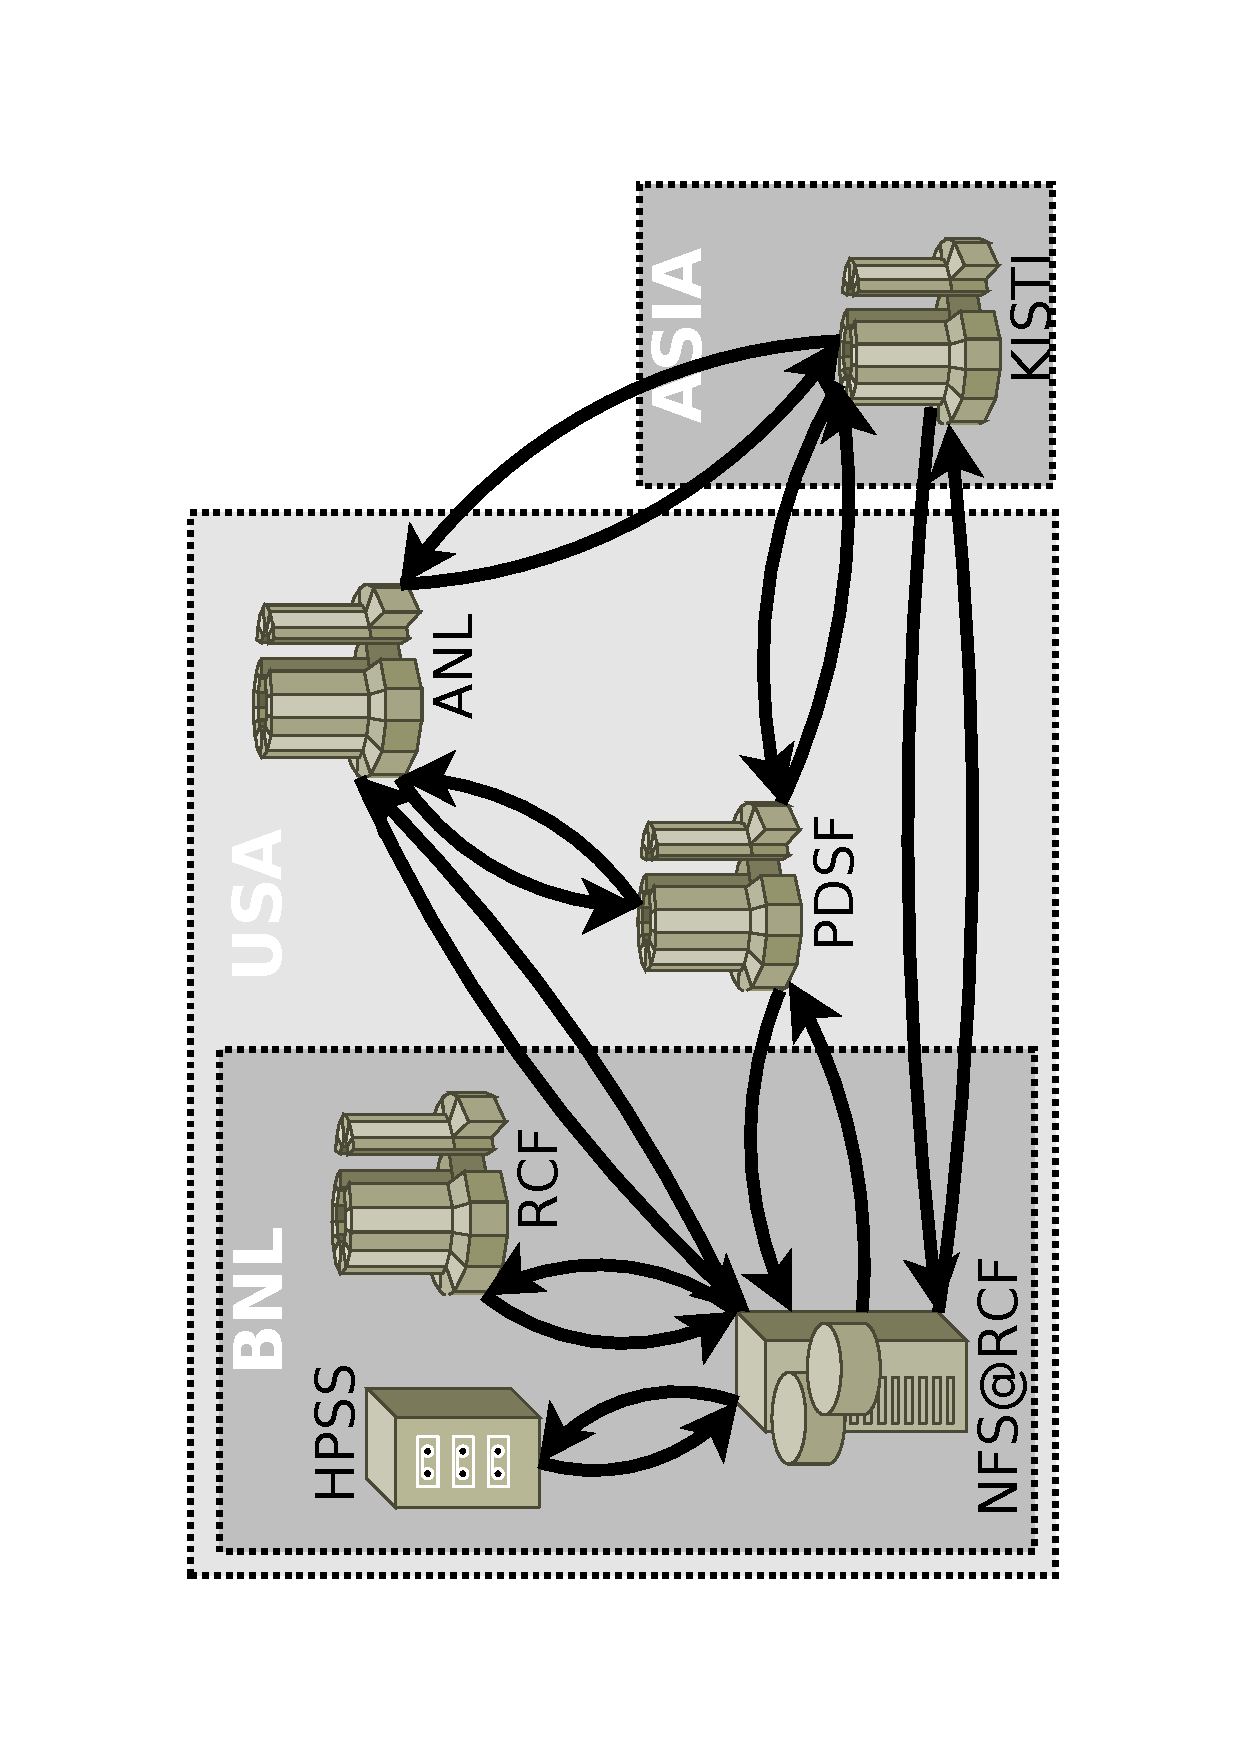
\includegraphics [trim= 30mm 30mm 30mm 30mm , clip, angle =-90, width=0.7\textwidth]{pic/sites.pdf}
	\end{center}
	\caption{Data production Grid of the experiment STAR. Raw data is recovered from central HPSS to NFS storage at RCF and then it is distributed between local and remote sites. Arrows represent network links.}
	\label{sites}
\end{figure} 	

When running data intensive applications on distributed computational resources long I/O overheads may be observed as access to remotely stored data is performed. Latency and bandwidth can become the major limiting factors for the overall computation performance and can reduce the CPU time\,/\,wall time ratio due to excessive I/O wait \cite{Betev,HorkyACAT}.  Widely used data management systems in HENP community (Xrootd \cite{Xrootd}, DPM \cite{DPM}) are focused on providing heterogeneous access to distributed storage and do not consider data pre-placement with respect to available CPUs, job durations or network performance. At the same time job scheduling systems (PBS, Condor) do not reason about transfer overheads when accessing data at distributed storage. For this reason, an optimization of data transferring and distribution across multiple sites is often done manually, using a custom setup for each particular infrastructure \cite{Balewski}.

Previous collaborative work between BNL (Brookhaven National Laboratory) and NPI/ASCR (Nuclear Physics Institute, Academy of Sciences of the Czech Republic) showed that the global planning of data transfers within the Grid can outperform widely used heuristics such as Peer-to-Peer and Fastest link (used in Xrootd)\cite{Zerola}. This concept was later complimented with usage of caching \cite{Makatun_cache}. The comparison and selection of the most appropriate caching policies for the data access pattern in HEP is described in Section \ref{Cache}. 
 
Those results became the ground for continuation of research and extension of global planning to the entire data processing workflow, i.e., scheduling of CPU allocation, data transferring and  placement at storage \cite{ACAT_cp,MISTA}. In Section \ref{CP_approach} we propose a constraint programming planner that schedules computational jobs and data transfers in a distributed environment in order to reduce the overall completion time. Since such global scheduling is computationally demanding it should be divided into several stages in order to improve scheduler performance and scalability. A planing of resource load can be accomplished in the first stage before scheduling particular file transfers and jobs. In Section \ref{Network_flow} we address the problem of data production planning, answering the question how the load should be distributed over resources and how the data should be transferred given the network structure, bandwidth, storage and CPU slots available. This will allow each computational site to load the CPUs with jobs while not exceeding disk and network capacities.

\subsection{Workload types}
Due to a data level of parallelism a typical workflow of HENP computation
consists of independent jobs requiring one CPU,  using one input and producing one output file each. This workload can be further divided into two classes of jobs: data production and user analysis.

Data production jobs are processing raw detector data into reconstructed physical events. This jobs are usually submitted centrally. Input files for these jobs are initially placed at the central data storage of an experiment (e.g. tape storage at Tier-0 site). Each raw file has to be processed once. An output file is of comparable size with the input file. After processing, the output file has to be copied back to the central storage. The typical task of a data production campaign would be to process a given dataset (i.e. several Petabytes of similar files) as soon as possible (e.g. next several month). Under such scenario the particular order of jobs is unimportant, while the makespan becomes the main value for an optimization. Since all the jobs processing input files form the same dataset are similar, parameters of upcoming jobs can be estimated knowing the statistics of completed jobs.

User analysis consists of jobs submitted by many different researches. These jobs are processing the reconstructed data which are the result of data production. Input files can have several copies within Grid. In this case the same input file can be processed several times by the same or different users. Output size of user analysis is negligible compared to the size of input. Each researcher uses its own code for analysis, for that reason the job parameters are far less predictable then for the data production. Moreover, when users submit their jobs to the batch system they often overestimate the runtime  to prevent their jobs being killed due to overrun.  Another contrast to data production is that the order of job execution plays an important role in user analysis - it defines so called \textit{fairness to users}. There is no strict definition of fairness in scheduling, but the general principle is that all the users should receive a fair share of resources. There exist several commonly accepted metrics to measure the quality of a schedule in a multi-user environment: response time, wait time, slowdown, fragmentation and etc. \cite{Rudova_Tabu_search}. 

Sections \ref{Network_flow} and \ref{CP_approach} are focused on scheduling for data production, while Section \ref{Cache} compares caching strategies for a user access pattern. 

\subsection{Usecases}
Long I/O overheads when accessing data from remote site can significantly reduce the application's CPUtime/WallTime ratio \cite{HorkyACAT,Betev}. For this reason, when setting up a data production at remote sites one has to consider the network throughput, available storage and CPU slots. When there are few remote sites involved in the data processing, the load can be tuned manually and simple heuristic may work, but, as the number of sites grows and the environment is constantly changing (site outage, fluctuations of network throughput and CPU availability), an automated planning of workflows becomes needed. 

As an intuitive example of optimization let us consider a situation when a given dataset can be either processed locally, or can be sent to a remote site. Depending on transfer overhead it may appear to be optimal to wait for free CPU slots at the local site and process all the data there, or send a smaller fraction of the dataset for remote processing. Commonly used heuristics such as ``\textit{Pull a job when a CPU slot is free}'' will not provide an optimization with respect to an overall processing makespan.  

Another example arises from a workflow optimization which was done for inclusion of the ANL (Argonne National Laboratory) computational facility into the Cloud based data production of the STAR experiment \cite{Balewski}. In this case, and due to the lack of local storage at the site for buffering, the throughput of a needed direct on-demand network connection between BNL (New York) and ANL (Illinois) was not sufficient to saturate all the available CPUs at the remote site. An optimization was achieved by feeding CPUs at ANL from two sources: directly from BNL and through an intermediate site NERSC (National Energy Research Scientific Computing Center, California) having large local caching and with better connectivity to ANL (see Figure \ref{sites}). This example illustrates an efficient use of indirect data transfers which cannot be guessed by simple heuristics. A general illustration of distributed resources used for data production and their interconnection is given at Figure \ref{fig:simulated grig}.

\begin{figure}[h]
\centering
    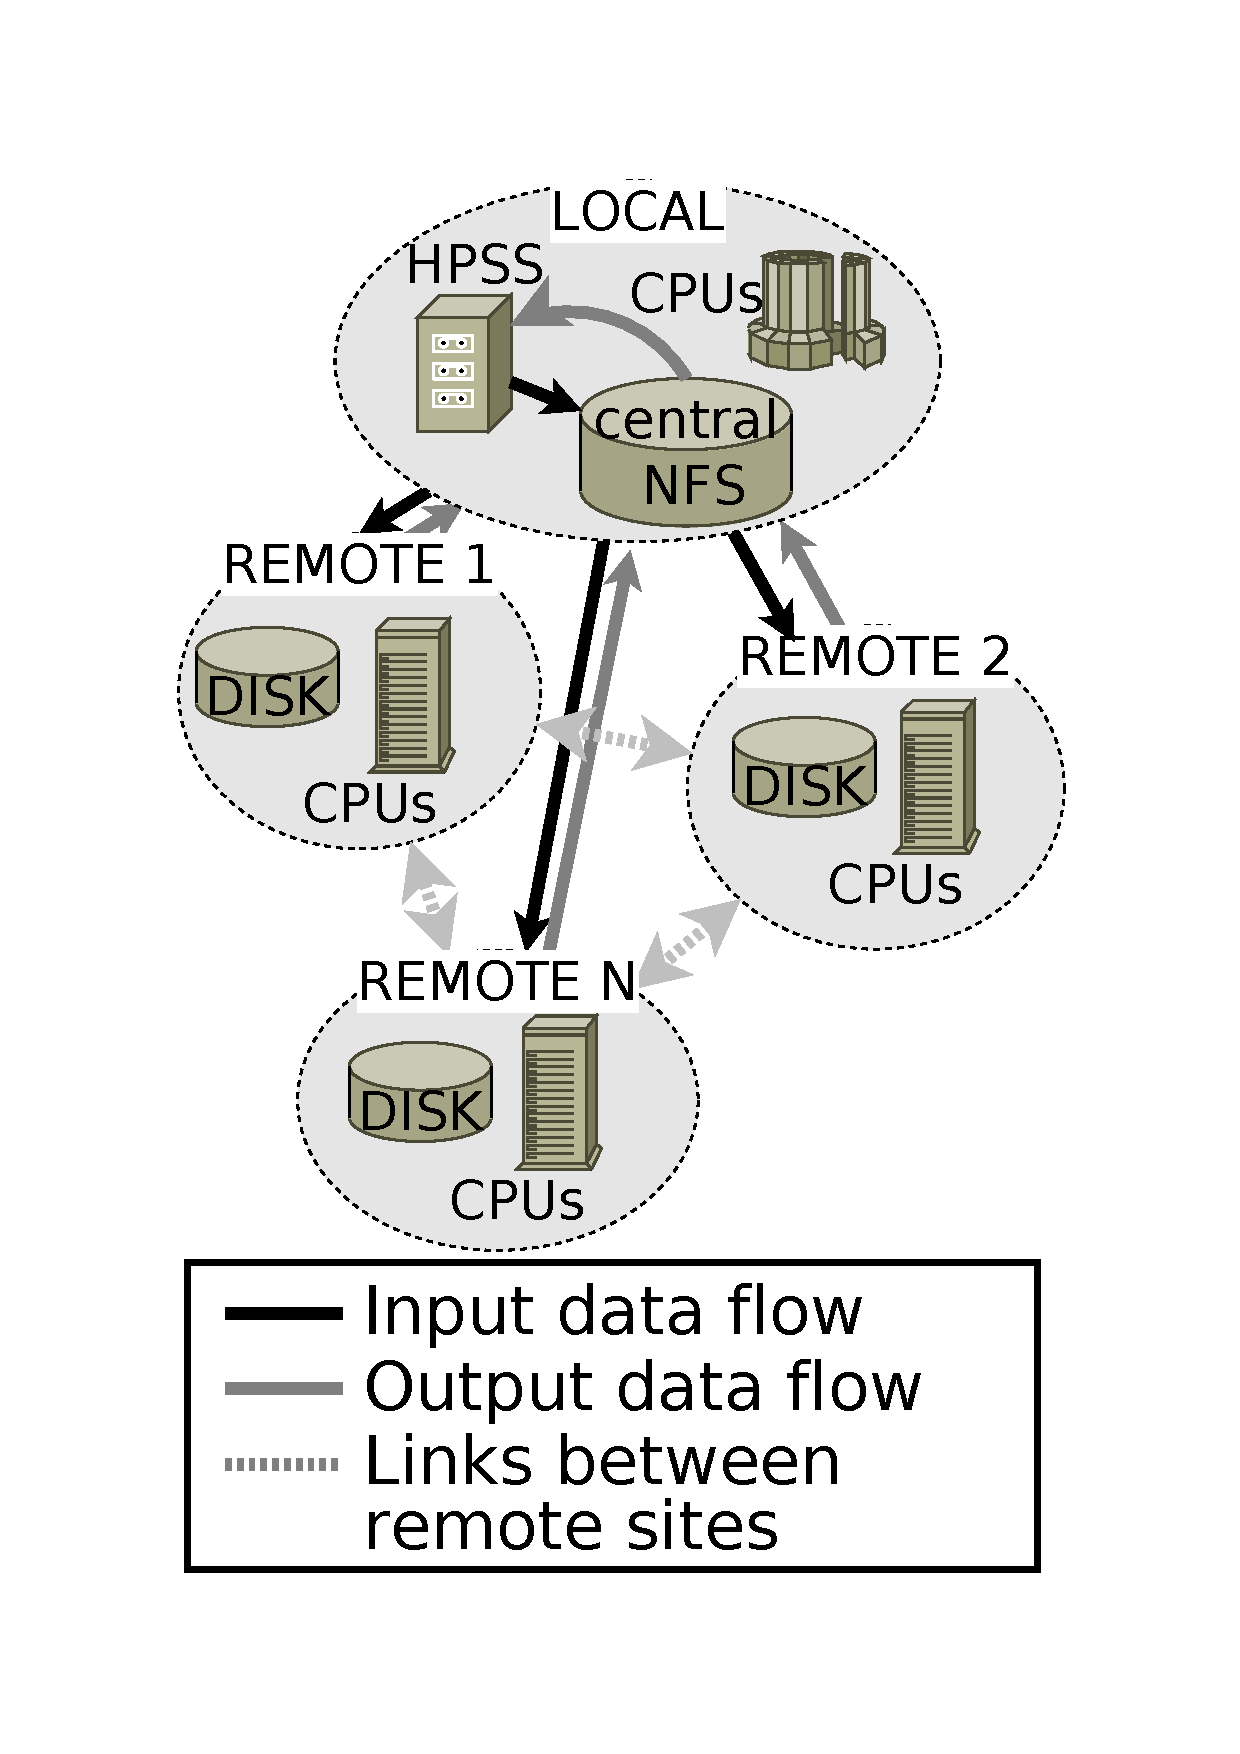
\includegraphics[trim =30mm 30mm 30mm 30mm ,clip, width=.4\textwidth]{pic/Data_production_general_bw2.pdf}
    \caption{Schema of data production in the Cloud.}
    \label{fig:simulated grig}
\end{figure}

Scheduling of computational jobs submitted by users (user analysis) has even more degrees of possible optimization: selection between multiple data sources, grouping of jobs that use the same input files. This case becomes even more complex due to a poor predictability of the user analysis jobs. However,  the main question for optimization remains the same as for the examples above: How to distribute a given set of tasks over the available set of resources in order to complete all the tasks within minimal time?

\subsection{Related work}
Most of the widely used job scheduling policies such as First Come First Served (FCFS), conservative backfilling (CONS), aggressive backfilling (EASY), selective backfilling and etc. \cite{srinivasan2002selective} are focused on maximizing CPU throughput and fairness to users. In work  \cite{Rudova_Tabu_search} the backfilling is performed with the help of Tabu search, which helps to find a schedule closer to the global optimum. In work \cite{Rudova_Multi-resource} authors proposed a multi-resource aware user prioritization mechanism, where fairness to users is improved by taking into account the usage of several resources (such as CPU, RAM, HDD, GPU) and heterogeneity of the system.  The above strategies are dedicated to manage a single computational cluster where data transfer overhead is not a significant factor. Also, for the data production workflow such metrics as fairness to users is irrelevant.
 
%Add Suffarage stratage, DAG schedulling 

In \cite{casanova2000heuristics} authors have modified existing heuristics  to schedule parameter sweep applications with file I/O requirements (e.g. Monte Carlo simulations), and studied an impact of inaccurate performance prediction on scheduling. Authors consider job scheduling on heterogeneous resources (Grid) taking data transfer overhead for each job into account. While the input transfer overhead was estimated knowing an end-to-end connection speed, the file transfers itself were not scheduled at network links, neither actual network topology was taken into account. In case of data production in HENP, uncoordinated data transfers may overcome the network capacity which leads to overall degraded performance. For this reason in our research we consider network load planning.

Optimization of data intensive applications in Grid was studied
in~\cite{Globus_scheduler}. In this work an optimization was achieved by
replication of highly used files to more sites while the jobs were executed
where their input data is located. However, this is not the case for data
production, when each file has to be processed once. 

Explicit model distributing jobs over a Grid with respect to the network
bandwidth was proposed in~\cite{Trees}. The network structure of the Grid was
modeled as a tree and all the files were assumed to be of the same size and
processing time. In our study we do not limit the network topology to trees,
and assume fluctuations of job parameters. 



\section{Resource load planning}
\label{Network_flow}
Due to a data level of parallelism a typical workflow of HENP computation
consists of independent jobs using one CPU, one input and one output file. For the following model we assume there is a local scheduler running at each site, which picks a new
input file to process from the local storage of that site each time when a CPU becomes
free. Input data must be transferred from the central storage
to each site in such a manner that at the every moment of time there is enough
input files at each site to keep all the available CPUs busy while not
exceeding the local storage and network throughput. Another task
is to transfer the output files back to central storage, cleaning each local
storage for the new input.

Let us consider a scheduling time interval $\Delta T$. We assume that at the
starting moment all the CPUs in the Grid are busy, and there is some amount of
input data already placed at each site. We need to transfer the next portion
of data to each site during time interval $\Delta T$ in order to avoid
draining of the local queue by the end of this interval. 

The computational Grid is represented by a directed weighted graph where
vertexes $c_{i} \in C$ are computational nodes and edges $l_{j} \in L$ are
network links. Weight of each link $b_{j}$ is the amount of data that can be
transferred over the link per unit of time (i.e. bandwidth). One of the nodes
$c_{0}$ is the central storage where all the input files for the further
processing are initially placed. All the output files has to be transferred
back to $c_{0}$ from the computational nodes. We will give two separate
problem formulations: for an input and output transfer planning. 

In order to formulate a network flow maximization problem \cite{Network_flows}
for input/output file transferring we have to define a capacitated $\{s,t\}$
network, which is a set of vertexes $V$ including a source $s$ and a sink $t$;
and a set of edges $e\in E$ with their capacities $cap(e)$. A solution that
assigns a nonnegative integer number $f(e)$ to each edge $e \in E$ can be
found in polynomial time with known algorithms.

\subsection{Input flow planning}
\label{inproblem}

\begin{figure}[h]
	\begin{center}
		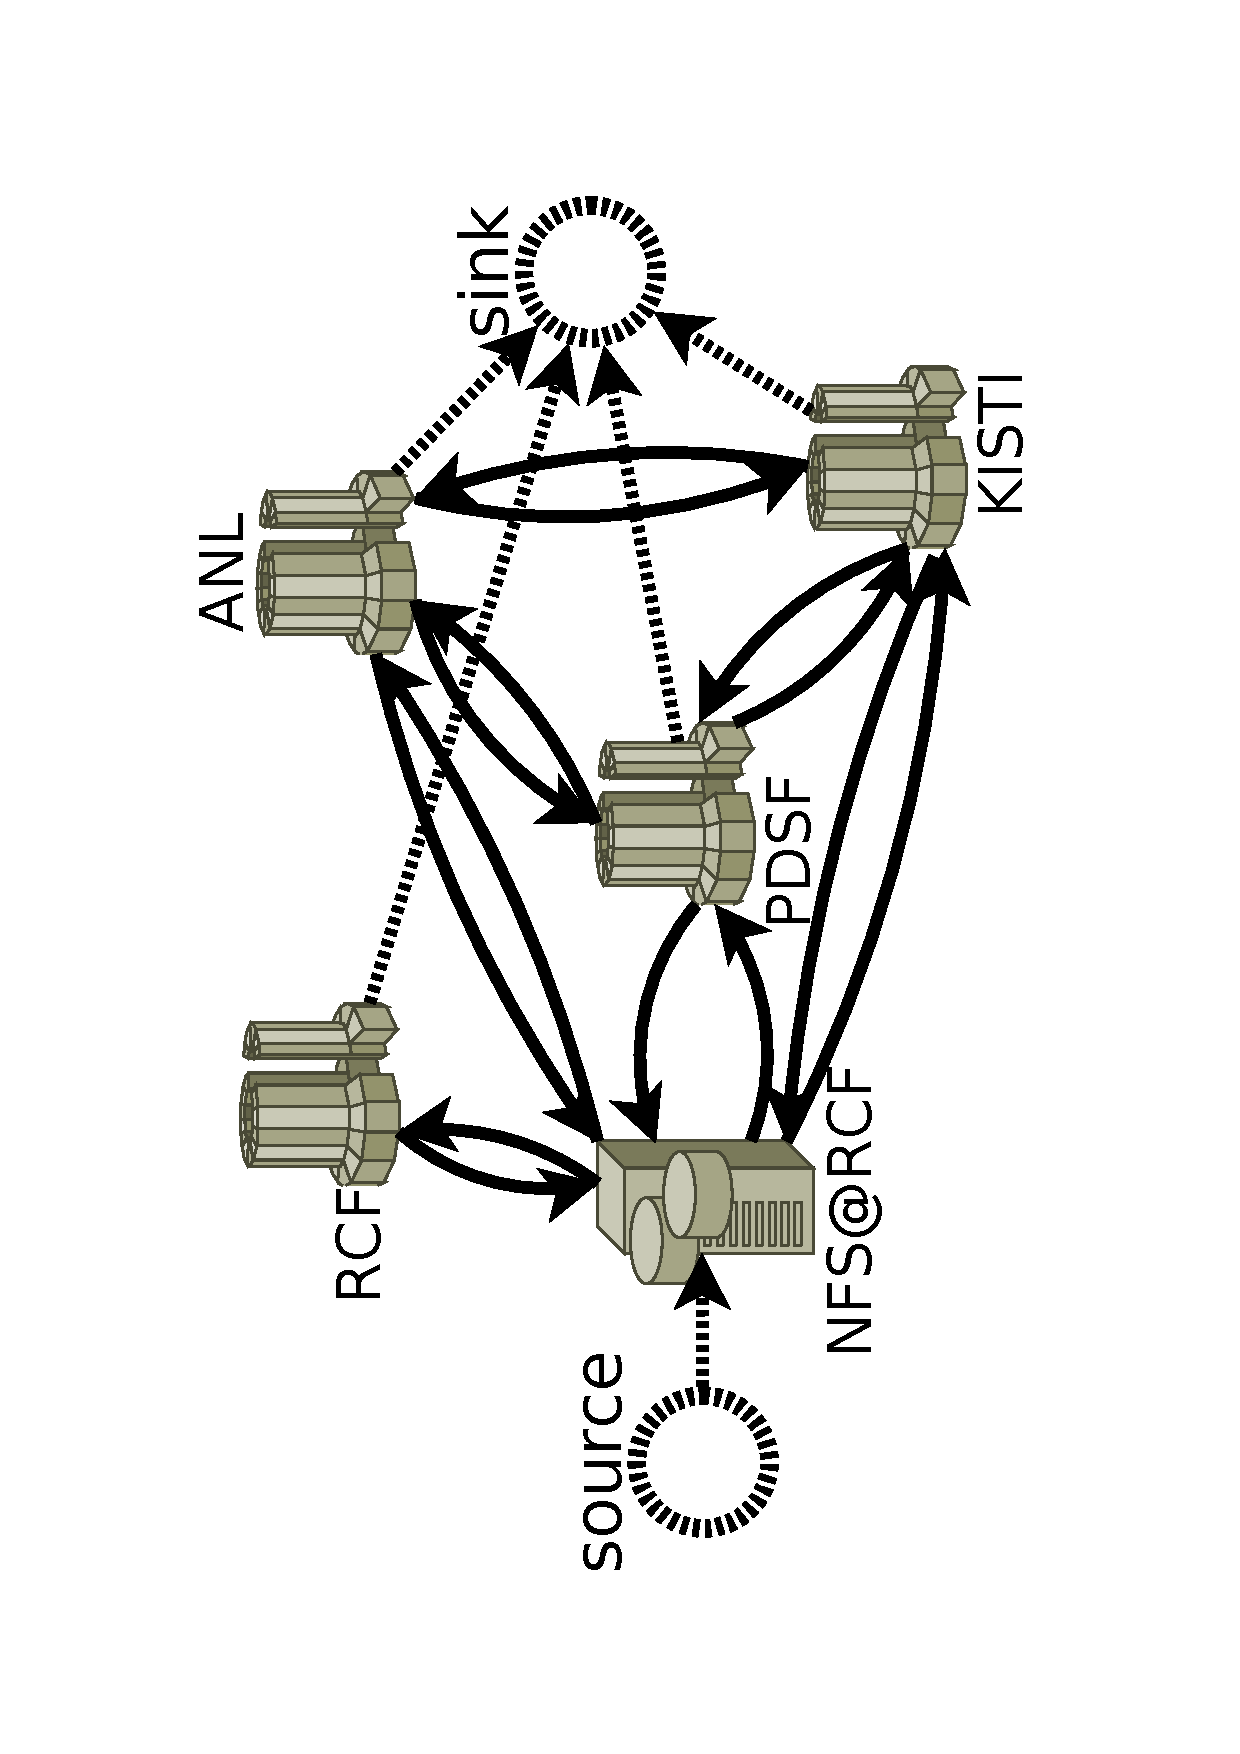
\includegraphics [trim= 30mm 30mm 30mm 30mm , clip, angle =-90, width=0.7\textwidth]{pic/real_network.pdf}
	\end{center}
	\caption{Input transfer planning: transformation of Data production Grid into   capacitated $\{s,t\}$ network for a flow maximization problem. Dummy vertexes (a source and a sink) are added. Each computational site is connected to the sink by a dummy edge. The source is connected to the NFS at RCF via dummy edge. The dummy edges are used in order to express constraints on network flow imposed by storage capacity and number of CPUs at each site.  Central HPSS is removed from consideration.}
	\label{real_network}
\end{figure} 

\begin{figure}[h]
	\begin{center}
		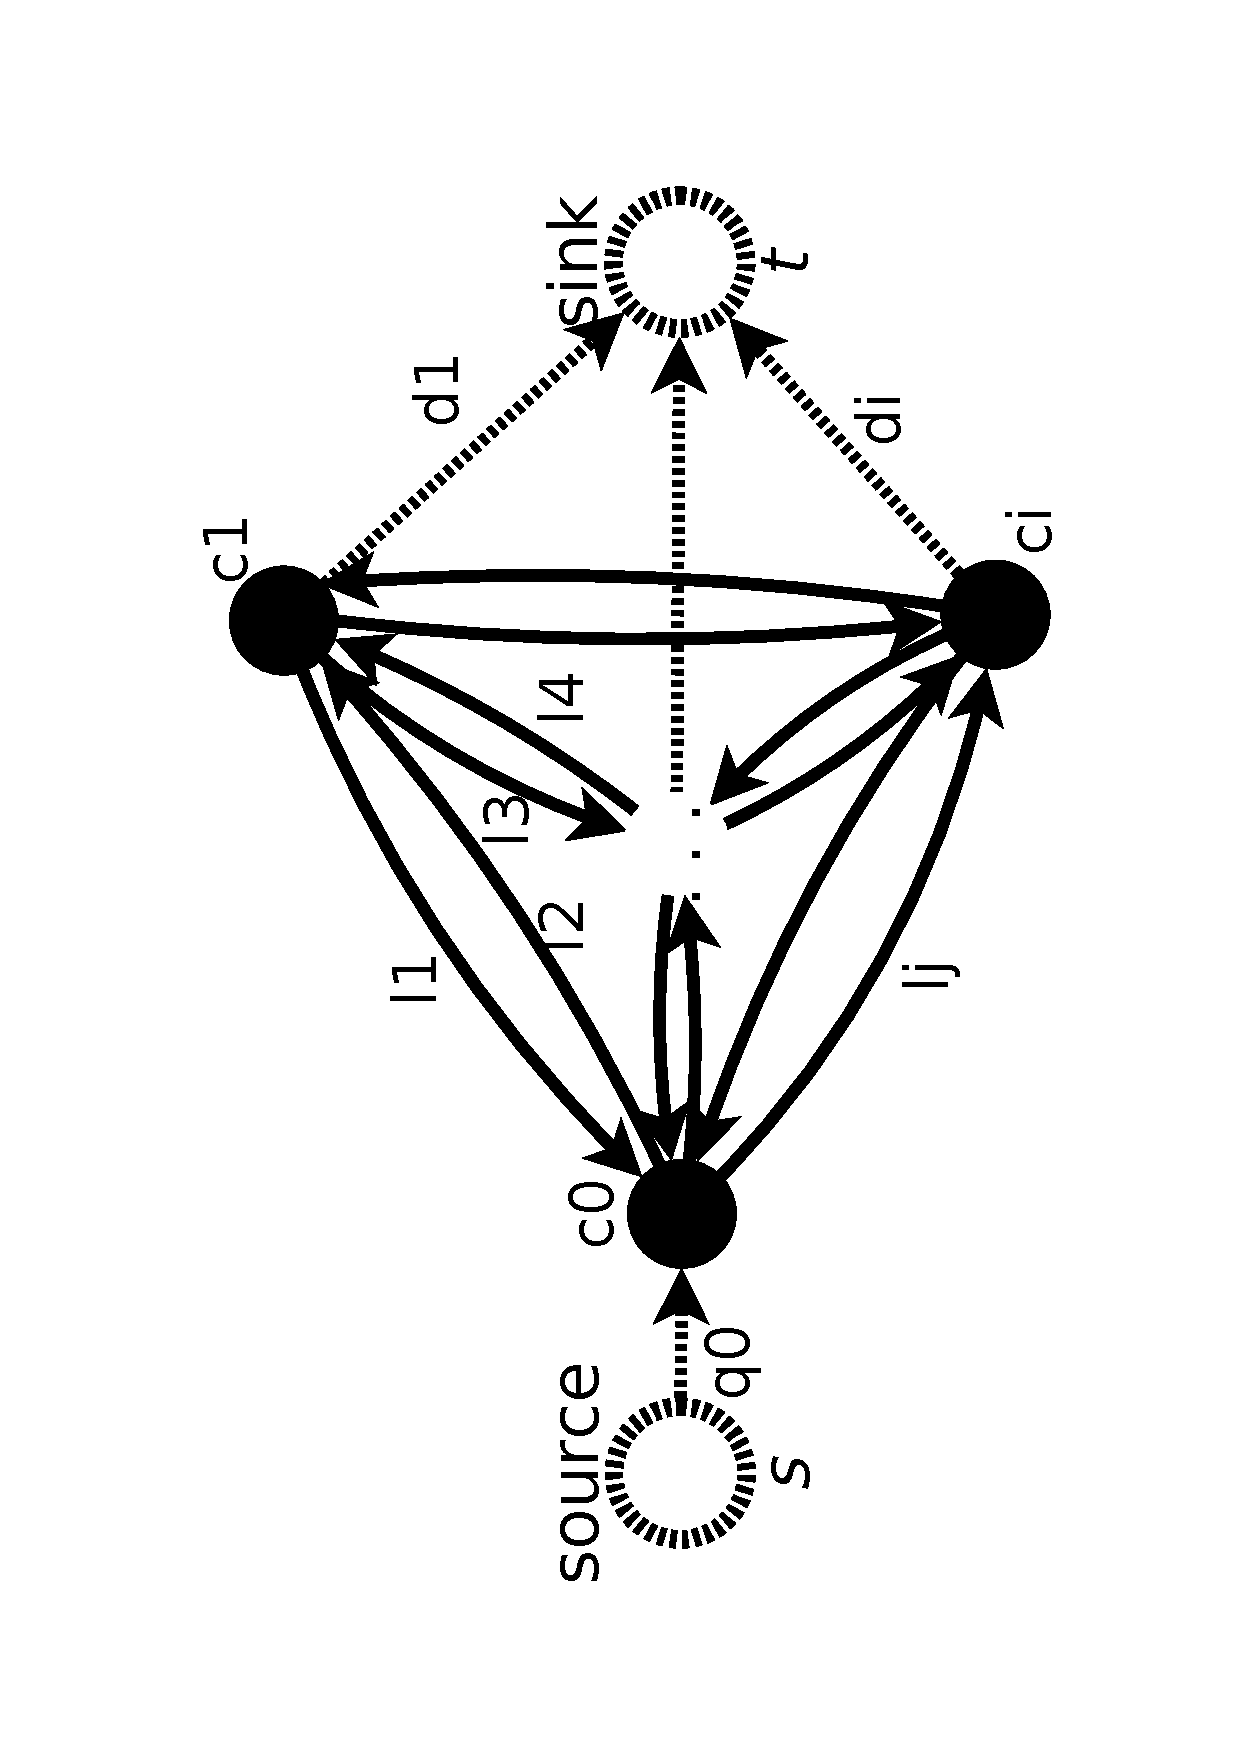
\includegraphics [trim= 30mm 20mm 30mm 30mm , clip, angle =-90, width=0.7\textwidth]{pic/network_general.pdf}
	\end{center}
	\caption{Data production Grid represented as an capacitated $\{s,t\}$ network for input transfer planning (general case). $c_{0}$ is a central NFS storage (Tier-0), $c_{i}$ are computational nodes (where $i>0$), $l_{j}$ are network links, $d_{i}$ are dummy edges from computational nodes to the sink $t$, $q_{0}$ is a dummy edge leading from the source $s$ to the $c_{0}$. }
	\label{network_general}
\end{figure} 

In order to transform a given graph of a Grid into a capacitated $\{s,t\}$
network for an input transfer problem we add two dummy vertexes: a source $s$
and a sink $t$. Next we add  dummy edges $d_{i} \in D$ from each computational
node $i$ to the sink, and a dummy edge $q_{0}$ from the source $s$ to the
central storage $c_{0}$.
For example, the transformation of the Grid form Figure \ref{sites} is illustrated at Figure \ref{real_network} (HPSS node was excluded from the consideration).


 These dummy edges allow us to introduce constraints
on the storage capacity of the nodes. The set of vertexes $V$ consists of
computational nodes $C$ and dummy vertexes: $V= C \cup \{s,t\}$. The final set
of edges consists of real network links $L$, dummy edges $D$ from
computational nodes to the sink and from the source to the central storage
$q_{0}$: $E= L \cup D \cup \{q_{0}\}$. Capacity of each edge defines the
maximal amount of data that can be transferred over an edge within time
interval $\Delta T$: 
%
\begin{equation} 
\label{edge_cap} 
cap(e) = \left\{
\begin{array}{l l} 
b_{j} \cdot \Delta T & \text{if }e = l_{j} \in L \\ w_{i} &
\text{if } e = d_{i} \in D\\ k_{0} & \text{if } e = q_{0} 
\end{array} \right.
\end{equation} 
%
where $w_{i}$ is the maximal amount of data that can be
transferred to the node $i$ without exceeding its storage capacity $Disk_{i}$
and $k_{0}$ is the total size of available input files at $c_{0}$. A general case of a resulting network in represented at Figure \ref{network_general}. We denote
the solution for the input transfer problem as $f^{in}(e)$.

\subsection{Output flow planning}
\label{outproblem}
\begin{figure}[h]
	\begin{center}
		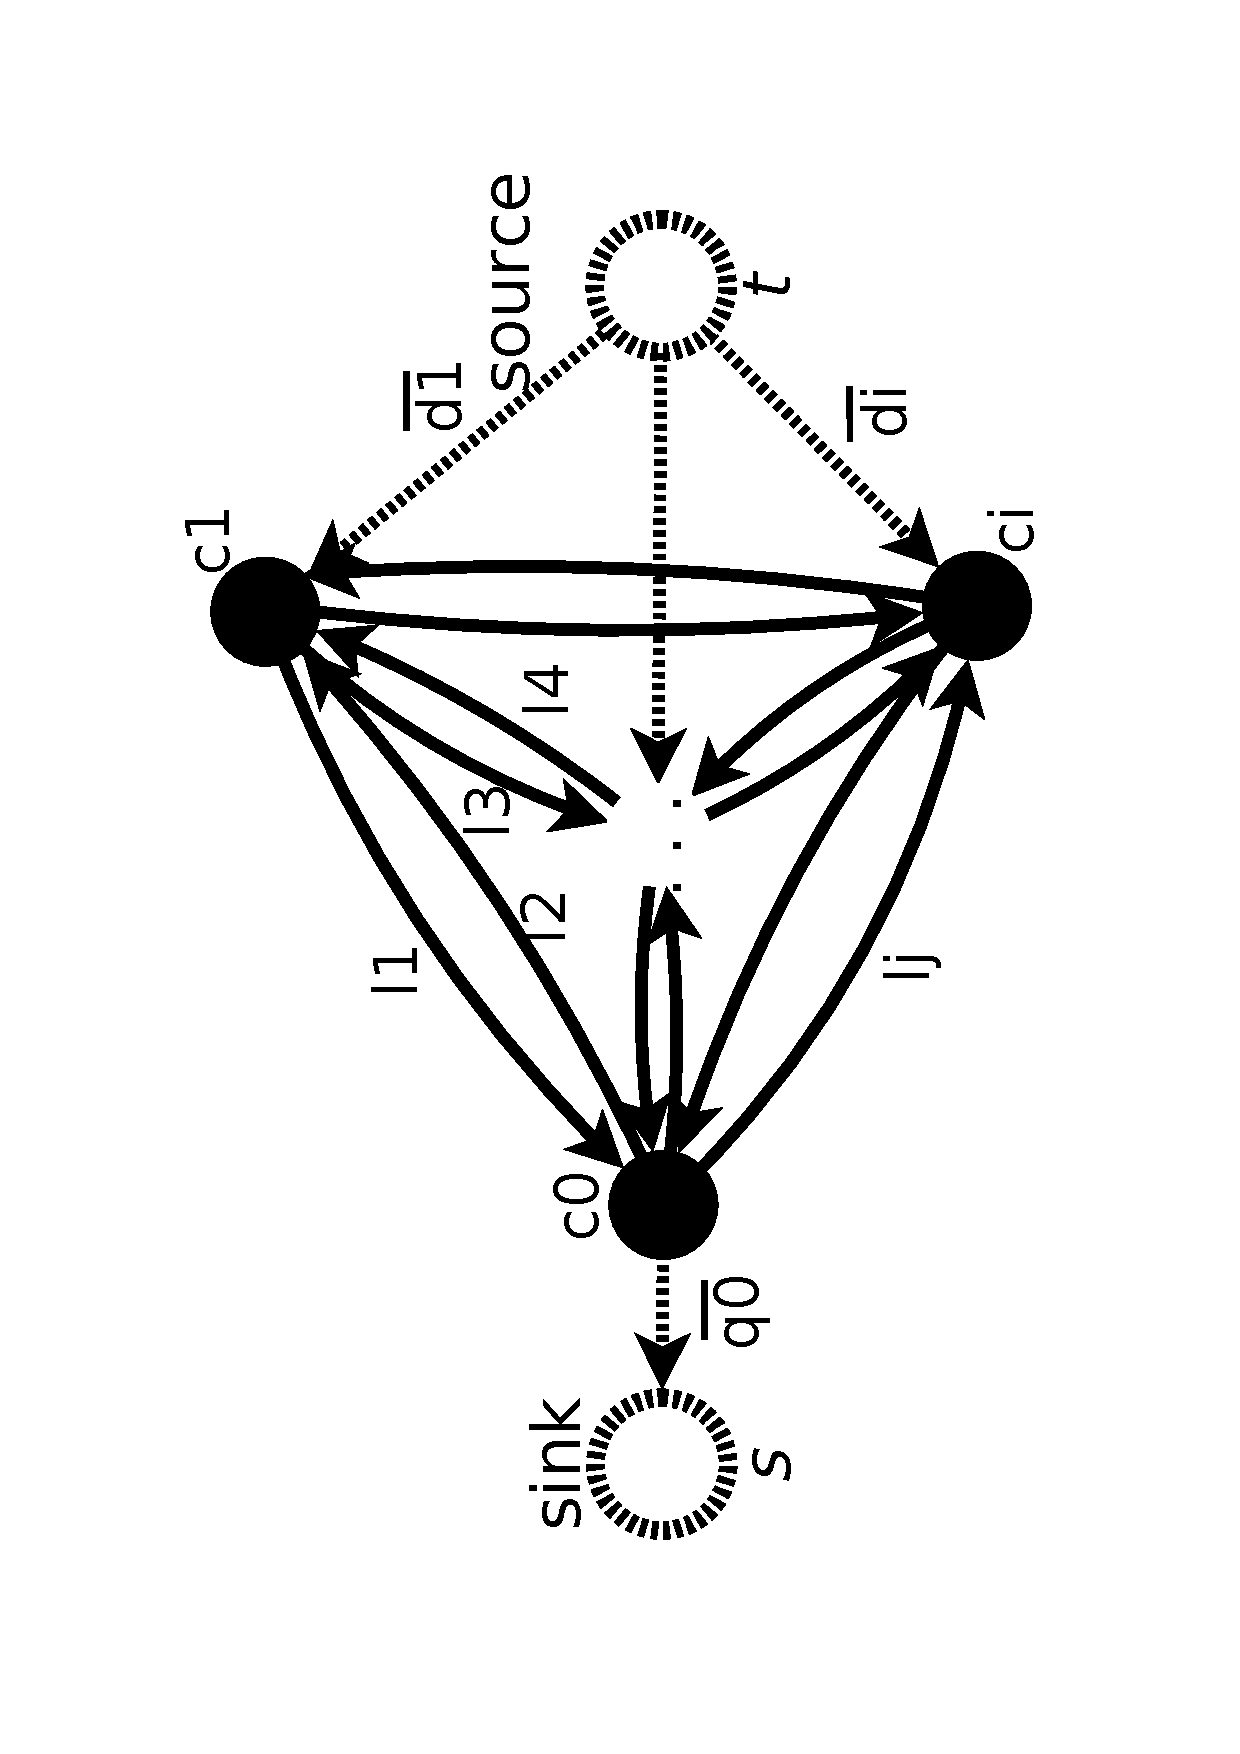
\includegraphics [trim= 30mm 20mm 30mm 30mm , clip, angle =-90, width=0.7\textwidth]{pic/network_general_out.pdf}
	\end{center}
	\caption{Data production Grid represented as an capacitated $\{t,s\}$ network for output transfer planning (general case). $c_{0}$ is a central NFS storage (Tier-0), $c_{i}$ are computational nodes (where $i>0$), $l_{j}$ are network links, $\overline{d}_{i}$ are dummy edges from the source $t$ to computational nodes, $\overline{q}_{0}$ is a dummy edge leading from $c_{0}$ to the sink $s$. }
	\label{general_out}	
\end{figure}

For transfer of output files we use a similar transformation, but swap the
source $s$ and the sink $t$, change the direction of dummy edges and redefine
capacities of dummy edges (see Figure \ref{general_out}). In this case the capacity $\overline{k}_{0}$ of the
dummy edge $\overline{q}_{0}$ leading from the central storage $c_0$ to the
sink $s$ is equal to the amount of data which can be transferred to $c_0$
within time interval $\Delta T$ (it is limited by the available space at the
central storage). The capacity $\overline{w}_{i}$ of dummy edges
$\overline{d}_{i}$ leading from the source $t$ to computational nodes $c_{i}$
is equal to the maximum amount of output data which can be transferred from
the node $c_{i}$.
%
\begin{equation}
\label{edge_cap_out}
cap(e) = \left\{ 
  \begin{array}{l l}
    b_{j} \cdot \Delta T & \text{if }e = l_{j} \in L \\
    \overline{w}_{i} & \text{if } e = \overline{d}_{i} \in \overline{D}\\
    \overline{k}_{0} & \text{if } e = \overline{q}_{0}
  \end{array} \right.
\end{equation}
%
We denote the solution for the output transfer problem as $f^{out}(e)$.

\subsection{Calculating capacity of dummy edges}
\label{dummycap}
Let us consider data production jobs which perform the same type of processing on the same type of files.
Duration $p_{j}$ of job $j$  processing input file of size $InSize_{j}$ at node $i$ is
\begin{equation}
\label{alpha}
p_{j} = \alpha_{i} \cdot InSize_{j} 
\end{equation}
Figure \ref{alpha-distr} shows a distribution of parameter $\alpha$ for 7000 of data production jobs executed at the same computational site (KISTI). It can be observed that the narrow peaks correspond to jobs using input files of the different type (\texttt{"st\_physics", "st\_physics", "st\_physics\_adc", "st\_jet"}, etc.). For this reason, parameter $\alpha$ can be considered constant for a given type of data processing at a given site. 

\begin{figure}[h]
	\begin{center}
		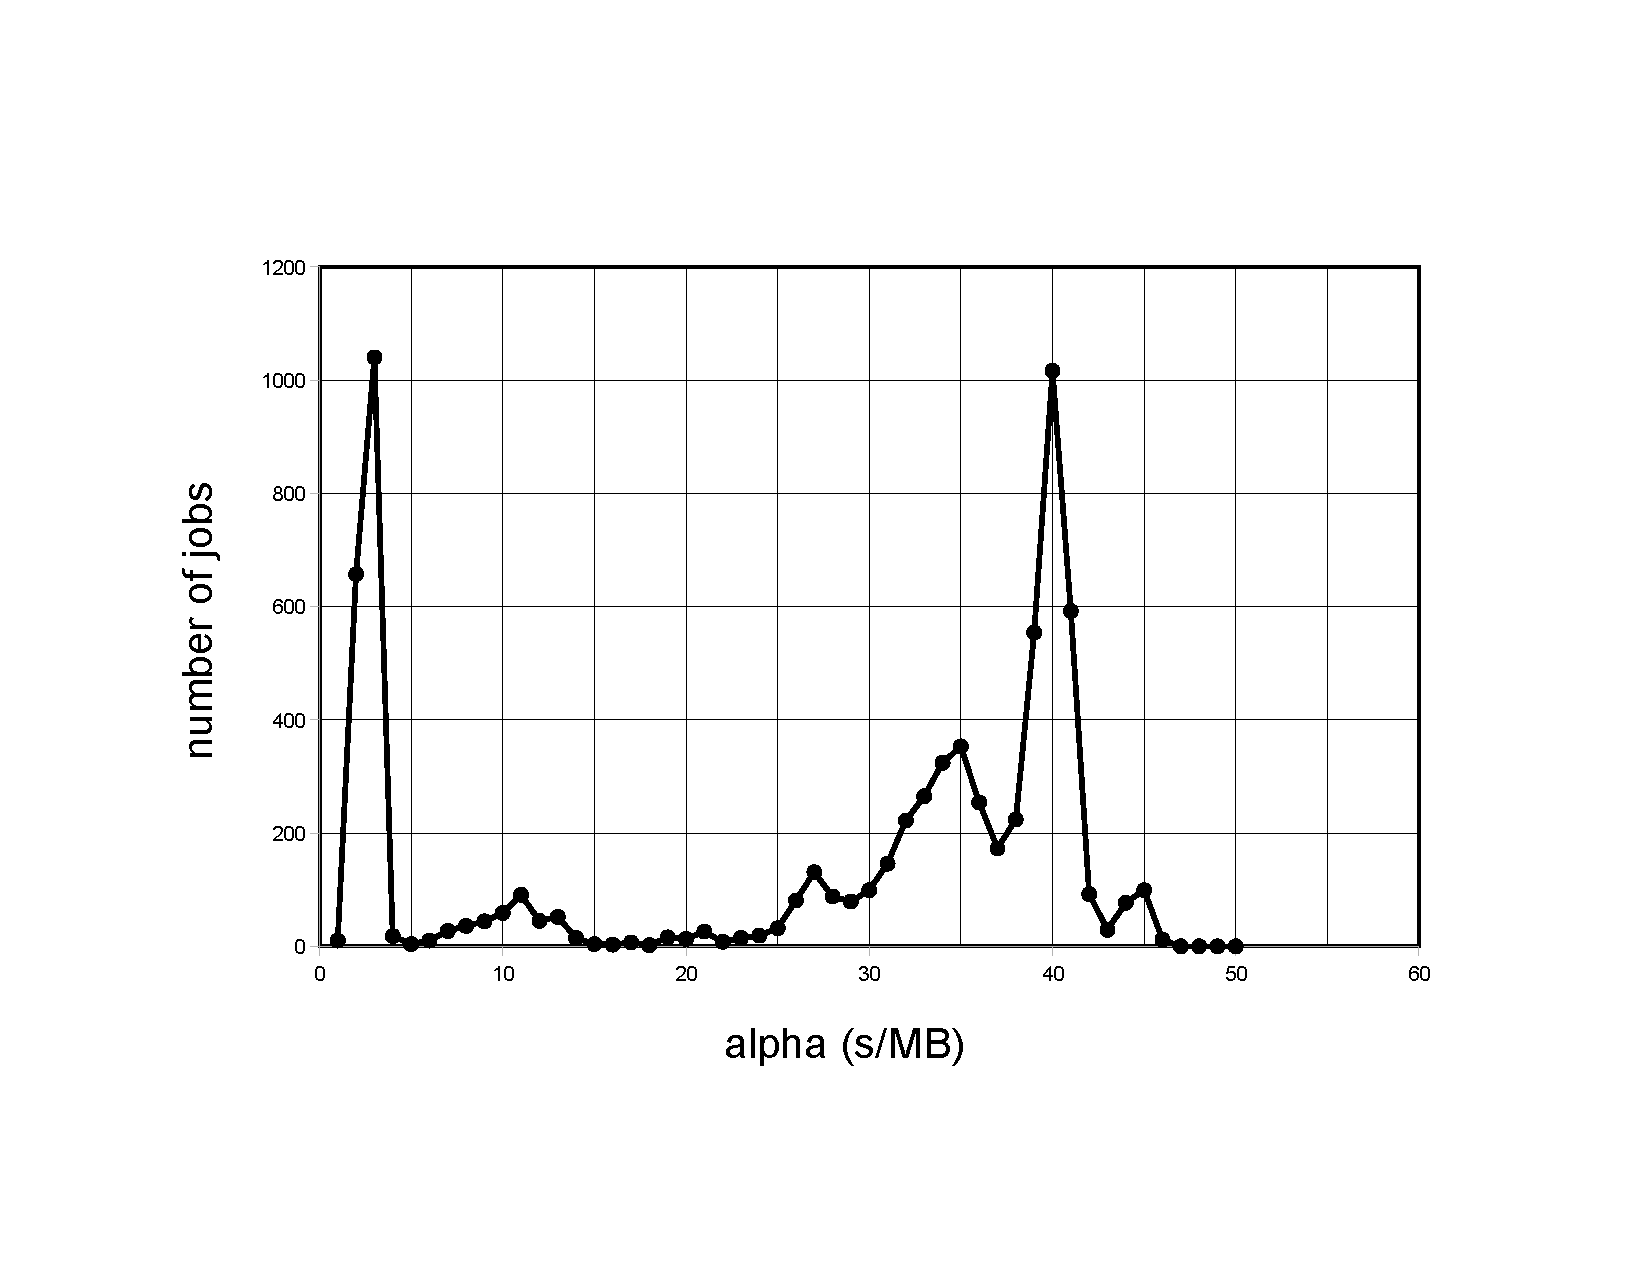
\includegraphics [trim= 20mm 30mm 10mm 30mm , clip, width=0.7\textwidth]{pic/alpha.pdf}
	\end{center}
	\caption{Distribution of parameter $\alpha$ (job duration divided by input file size) calculated for sample of 7000 jobs executed at KISTI during June - September 2014. Narrow peaks correspond to jobs using input files of different types (\texttt{"st\_physics"} at 40 s/MB, \texttt{"st\_physics\_adc"} at 3 s/MB, \texttt{"st\_jet"} at 35 s/MB, etc.). For this reason, parameter $\alpha$ can be considered constant for a given type of data processing.}
	\label{alpha-distr}
\end{figure} 

The ratio of size of input $InSize_{j}$ and output $OutSize_{j}$ files of each job $j$ is considered to be constant for the same type of data processing:
\begin{equation}
\label{beta}
OutSize_{j} = \beta \cdot InSize_{j} 
\end{equation}
Figure \ref{beta-distr} shows a distribution of parameter $\beta$ for 7000 of data production jobs executed at the same computational site (KISTI). Similarly to written above, for a given type of data processing this parameter can be considered constant. 

During time interval $\Delta T$ (which should be long enough) a node $i$ with number of CPUs $NCPU_{i}$ will process $\frac{1}{\alpha_{i}} \cdot NCPU_{i} \cdot \Delta T$ of input data and will produce $\frac{\beta}{\alpha_{i}} \cdot NCPU_{i} \cdot \Delta T$ of output data.

\begin{figure}[h]
	\begin{center}
		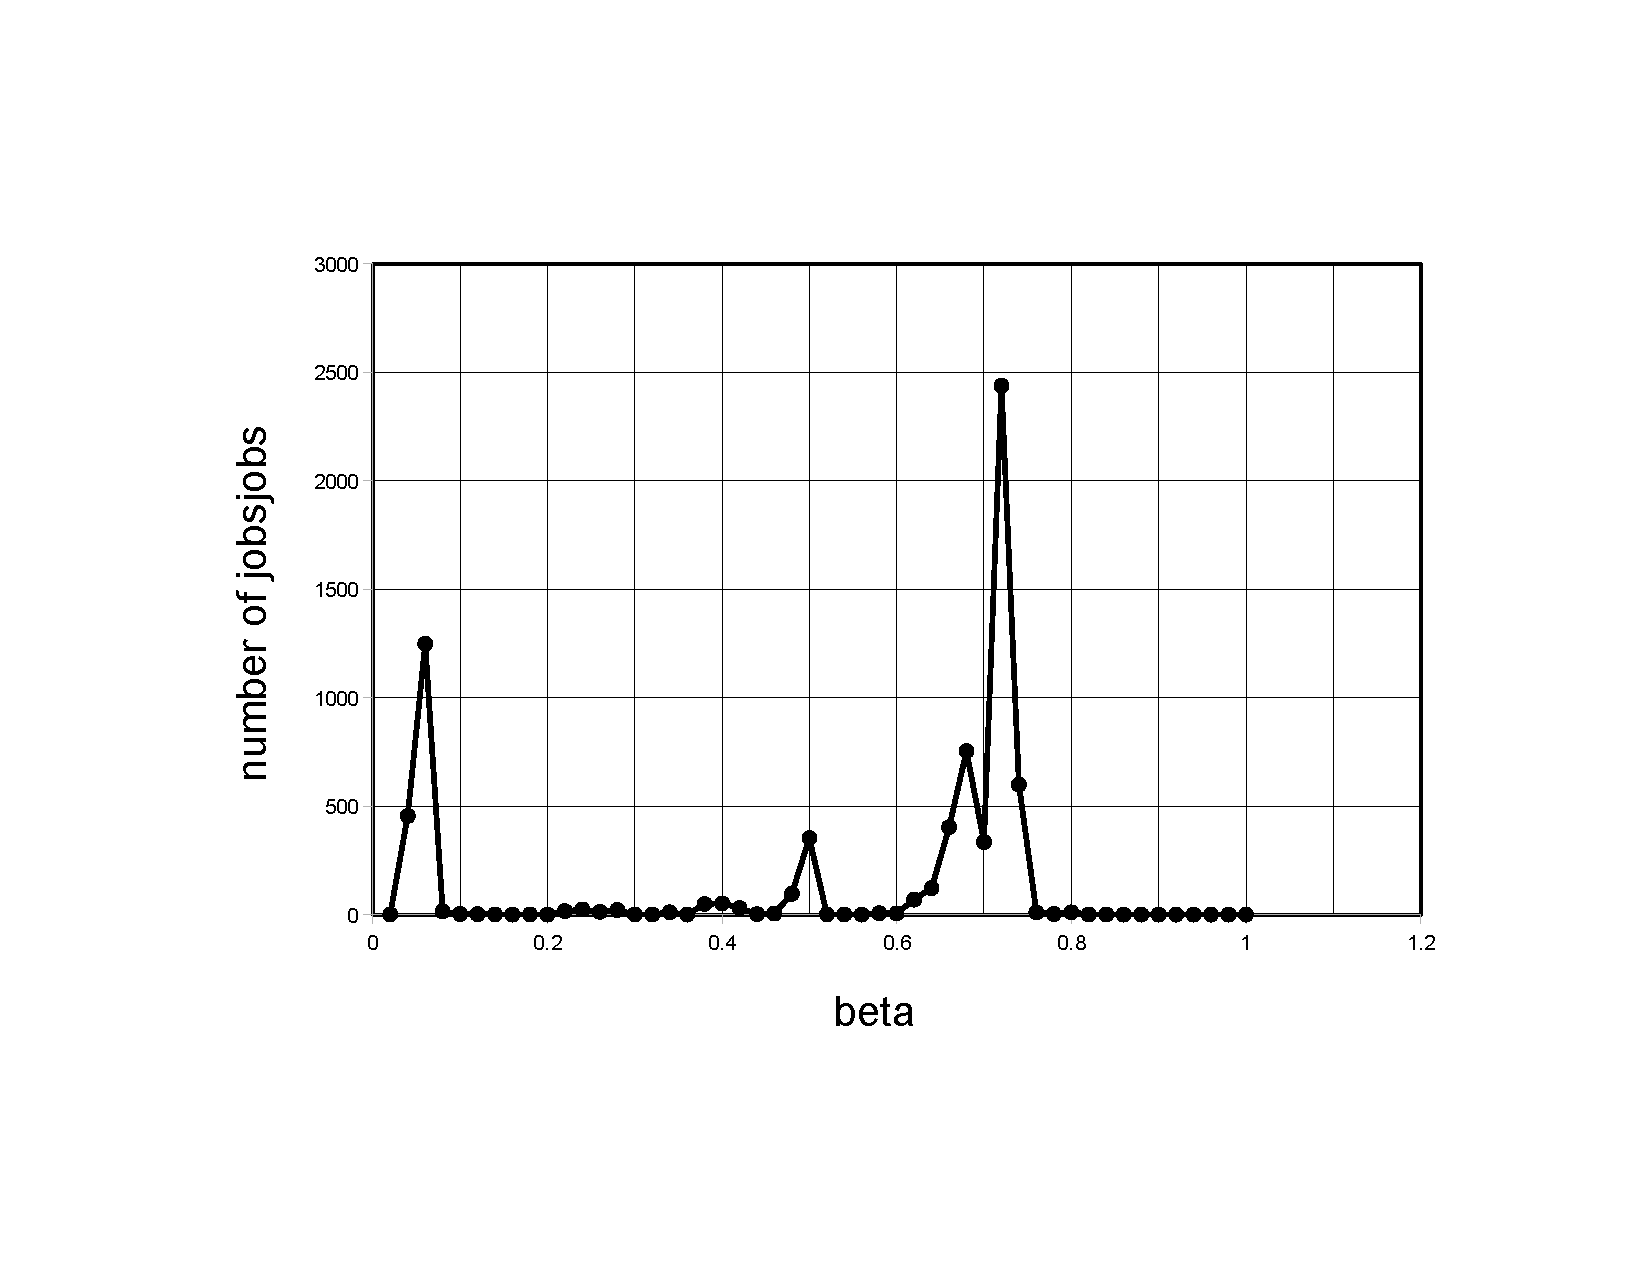
\includegraphics [trim= 20mm 30mm 10mm 30mm , clip, width=0.7\textwidth]{pic/beta.pdf}
	\end{center}
	\caption{Distribution of parameter $\beta$ (ratio of output file size over input file size) calculated for sample of 7000 jobs executed at KISTI during June - September 2014. Narrow peaks correspond to jobs using input files of different types (\texttt{"st\_physics"} at 0.72, \texttt{"st\_physics\_adc"} at 0.04, \texttt{"st\_fms"} at 0.5 , etc.). For this reason, parameter $\beta$ can be considered constant for a given type of data processing.}
	\label{beta-distr}
\end{figure} 

Let us consider a storage at a processing node $i$ during time interval $\Delta T$. 
$Disk_{i}$ is available disk space at node $i$.
The $I_{i}^{in}$ is the initial size of input data stored at the local storage;
$I_{i}^{out}$ is the initial size of output data at the storage; 
$New_{i}^{in}$ is the amount of input data that will be transferred to $i$ during $\Delta T$; 
$Del_{i}^{in}$ is the amount of input data that will be deleted from the storage, because the jobs using these input data will be completed; 
$Del_{i}^{out}$ is the amount of output data which will be deleted from the storage, because it will be transferred out of the node; 
$New_{i}^{out}$ is the size of new output files to be created during $\Delta T$;
$Min_{i}^{in}$ is minimal amount of input data (this includes input files of running jobs and files in the local queue to ensure stable CPU saturation), 
$Min_{i}^{out}$ - total size of output files which can not be transferred because the jobs which produce them are not finished (output files of running jobs). 

In the end of $\Delta T$ there should be enough input data to keep CPUs busy:
\begin{equation}
I_{i}^{in} + New_{i}^{in} - Del_{i}^{in} \geq Min_{i}^{in} \geq 0
\label{indata}
\end{equation}

In the end of $\Delta T$ the storage capacity should not be exceeded:

\begin{equation}
0 \leq I_{i}^{in} + I_{i}^{out} + New_{i}^{in} + New_{i}^{out} - Del_{i}^{in} - Del_{i}^{out} \leq Disk_{i}
\label{maxdisk}
\end{equation}

The balance of the output data at the end of $\Delta T$ is:
\begin{equation}
I_{i}^{out} + New_{i}^{out} - Del_{i}^{out} \geq Min_{i}^{out} \geq 0
\label{outdata}
\end{equation}

If the scheduling interval $\Delta T$ is long enough, then we can use the following approximation:
\begin{equation}
Del_{i}^{in} \approx \frac{1}{\alpha_{i}} \cdot NCPU_{i} \cdot \Delta T
\label{delIn}
\end{equation}
and
\begin{equation}
New_{i}^{out} \approx \frac{\beta}{\alpha_{i}} \cdot NCPU_{i} \cdot \Delta T
\label{newOut}
\end{equation}
Then, combining Equations \ref{indata}, \ref{maxdisk}, \ref{delIn} and \ref{newOut} we can estimate amount of new input data $New_{i}^{in}$ which can be transferred to a node.
\begin{equation}
Min_{i}^{in} + \frac{1}{\alpha_{i}} \cdot NCPU_{i} \cdot \Delta T - I_{i}^{in} 
\leq New_{i}^{in} \leq
Disk_{i} - I_{i}^{in} - I_{i}^{out} + \frac{1 - \beta}{\alpha_{i}} \cdot NCPU_{i} \cdot \Delta T + Del_{i}^{out}
\label{newIn}
\end{equation}

Similarly, using Equations \ref{outdata} and \ref{newOut} the amount of output data which can be deleted from a node is
\begin{equation}
\label{delOut}
Del_{i}^{out} \leq I_{i}^{out} + \frac{\beta}{\alpha_{i}} \cdot NCPU_{i} \cdot \Delta T - Min_{i}^{out}
\end{equation}  

Since $w_{i}$ was defined in Subsection \ref{in_problem} as maximal amount of input data that can be transferred to the computing node $c_{i}$, we can now define it using Equation \ref{newIn}:
\begin{equation}
w_{i} =
Disk_{i} - I_{i}^{in} - I_{i}^{out} + \frac{1 - \beta}{\alpha_{i}} \cdot NCPU_{i} \cdot \Delta T + Del_{i}^{out}
\label{w}
\end{equation}
where $Del_{i}^{out}$ is equal to the amount of data which will be transferred from node $c_{i}$, i.e. the solution to the output transfer problem $f^{out}(\overline{d}_{i})$ (see Subsection \ref{outproblem}). The other values used in Equation \ref{w} can be obtained from monitoring data.

Similarly, $\overline{w}_{i}$ was defined in Subsection \ref{outproblem} as maximal amount of output data which can be transferred from node $c_{i}$. From Equation \ref{delOut} we obtain:
\begin{equation}
\label{sigma}
\overline{w}_{i} = I_{i}^{out} + \frac{\beta}{\alpha_{i}} \cdot NCPU_{i} \cdot \Delta T - Min_{i}^{out}
\end{equation}  
where $\Delta T$,  $Min_{i}^{out}$ are parameters of the scheduler, and the rest of the values can be extracted from monitoring system.

\subsection{Disjoint input and output transfer}
In this subsection we will prove that maximum flow problems for input and output transfers can be solved independently under assumptions: (a) all the real network links in considered Grid are full-duplex, i.e. network throughput between two nodes is the same in both directions (b) in stable regime size of output transferred from each node is proportional to size of input transferred to that node at each scheduling interval, i.e. $f^{out}(\overline{d}_{i})= \beta \cdot f^{in}(d_{i})$, where $\beta \leq 1$.

Let us consider two distinct computational nodes $c_{1}$ and $c_{2}$ connected by two opposite directed links $l_{1}=(c_{1},c_{2})$ and $l_{2}=(c_{2},c_{1})$ with equal capacities $cap(l_{1})=cap(l_{2})$. If a solution of the input transfer problem assigns flows to this links such that $f^{in}(l_{1}) \geq f^{in}(l_{2}) > 0$ then we can substitute such solution $f^{in}(e)$ with a new one $\widehat{f}^{in}(e)$ where $\widehat{f}^{in}(l_{1}) = f^{in}(l_{1}) - f^{in}(l_{2})$, $\widehat{f}^{in}(l_{2}) = 0$ and flows over the rest of the links are unchanged. The same is true for output transfer. This proves that in an optimal solution the same type of files (input or output) are transferred between any two nodes in one direction only, i.e. over one of directed links only. 

If we have an optimal solution for the input flow maximization problem $f^{in}(e)$ we can produce from it an optimal solution for the output flow maximization problem $f^{out}(e)$ such that for any opposite pare of links $l_{1}=(c_{1},c_{2})$ and $l_{2}=(c_{2},c_{1})$ the output flow is $f^{out}({l_{1}}) = \beta \cdot f^{in}({l_{2}})$ and since $\beta < 1$ the capacity of links is not exceeded  $f^{out}({l_{1}}) =\beta \cdot f^{in}(l_{2}) \leq f^{in}(l_{2}) \leq cap(l_{2}) = cap(l_{1})$. Due to symmetry of the two problems, this solution  $f^{out}(e)$ is also the maximum flow for the output transfer problem. Combining this with what was proven in previous paragraph, if $f^{in}({l_{1}}) > 0$ then $f^{in}({l_{2}}) = 0$ and thus $f^{out}({l_{1}}) = 0$. This means that in the optimal solution input and output files are never transferred over the same link. And thus, maximum flow problems for input and output transfers can be solved independently. 


\subsection{Solving Procedure}
\label{solve}
The maximum flow problems for input and output transfers
can be solved independently under assumptions: (a) all the real network links
in the considered Grid are full-duplex, i.e., a network throughput between two
nodes is the same in both directions (b) in a steady state the size of the
output transferred from each node is proportional to the size of the input
transferred to that node in each scheduling interval, i.e.,
$f^{out}(\overline{d}_{i})= \beta \cdot f^{in}(d_{i})$, where $\beta \leq 1$.

Since in real environment the assumption (b) will not strongly hold due to
resource performance fluctuations we propose the following approach to
solve the problem:
%
\begin{enumerate}
\item Calculate values for $\overline{w}_{i}$ using Eqn.~\ref{sigma}.
\item Solve the problem for output data flows to obtain $f^{out}(e)$.
\item Using Eqn.~\ref{w} and $Del_{i}^{out} = f^{out}(\overline{d}_{i})$ calculate $w_{i}$.
\item For real links $l \in L$ reduce the capacity by the amount which is used by output transfers: $cap(l_{j}) = b_{j} \cdot \Delta T - f^{out}(l_{j})$.
\item Solve the problem for input transfers with $w_{i}$ and $cap(l_{j})$ defined in previous steps. Find input data flows $f^{in}(e)$.
\end{enumerate}
%
To conclude, this procedure is expected to compute feasible data transfers 
such that CPUs in Grid are busy with computational jobs while not exceeding 
local disk capacities.

\section{Constraint programming approach}
\label{CP_approach}
Problems of scheduling, planning and optimization are being commonly solved with the help of Constraint Programming (CP) \cite{CP}. It is a form of declarative programming which is widely used in scheduling, logistics, network planning, vehicle routing, production optimization etc... In the this section we will introduce our Constraint Satisfaction Problem (CSP) formulation for a data production at multiple sites and provide a simulation-based evaluation of the proposed model. In contrast to the model in previous section which plans global data flow this model describes per job/file/transfer scheduling. 

We will introduce only the core concepts of our CSP formulation and search algorithms, omitting  detailed mathematical expressions.
The following input parameters are necessary to define our CSP.
\begin{description}
\item[Computational Grid] (see Figure \ref{fig:simulated grig}) is described by directed weighted graph where nodes are computational sites $c$ with a given number of CPUs $cpu_{c}$ and storage space $disk_{c}$; edges are network links $l$ with weight $slowdown_{l}$ which is the time required to transfer a unit of data ($slowdown_{l}=\frac{1}{throughput_{l}}$). A dedicated storage facility, such as HPSS \cite{HPSS}, can also be modeled as a node with $cpu_{c}=0$.
\item[Set of jobs.] Each job $j$ has a $duration_{j}$, it needs one input file of $inputSize_{j}$, produces one output file of $outputSize_{j}$, input file is placed at $inputSourceNodes_{j}$ and output file must be transferred to one of $outputDestinationNodes_{j}$.
\end{description}
Our goal is to create a schedule of jobs at computational sites, transfers over links and a placement of files at storages for a given computational Grid and a set of jobs. In order to solve this problem the variables of our model define the \textit{resource selection} and  \textit{timing} of each task:
\begin{description}
\item[Resource selection variables] define a node $ProcessingNode_{j}$ where the job $j$ will be executed and a transfer path for each file $f$ (either input or output of a job). The transfer path is described by a set of boolean variables $X_{fl}$ where $true$ means that a file $f$ will be transferred over a link $l$ and $false$ means the opposite.
\item[Time variables] are: $Js_{j}$ is a start time of a job $j$, $Ts_{fl}$ is a start time of a transfer of a file $f$ over a link $l$, $Fs_{fc}$ is a start time of a placement of a file $f$ at a node $c$, $Fdur_{fc}$ is a duration of a placement of a file $f$ at a node $c$.
\end{description} 	 
 In our model we assume that a network link can be modeled as an unary resource with no loss of generality. The measurements in \cite{Zerola} have shown, that  a sequential transfer of a set of files does not require more time than a parallel transfer of the same set of files over the same link.

\subsection{Search overview}
We use an incomplete search which can provide a suboptimal solution of required quality within a given time limit because the final goal is to create a planner that can process requests online.
For a better search performance the overall problem is divided into two subproblems and the search is performed in two stages: 
\begin{enumerate}
\item Planning Stage: instantiate a part of variables in order to assign resources for each task.     
	\begin{enumerate}
	\item Assign jobs to computational nodes. 
	\item Select transfer paths for input and output files. 
	\item Estimate a makespan for a given resource assignment $estMakespan$.
	\item Find a solution for the subproblem with a minimal estimated makespan. 
	\end{enumerate}
\item Scheduling stage: define a start time for each operation. 
	\begin{enumerate}
	\item Define the order of operations. 
	\item Put cumulative constraints on resources in order to avoid their oversaturation at any moment of time.
	\item Find a solution with a minimal $makespan$ which is the end time of the last task. 
	\end{enumerate}
\end{enumerate}

\subsection{Constraints at the planning stage}
\begin{figure}[h]
\centering
    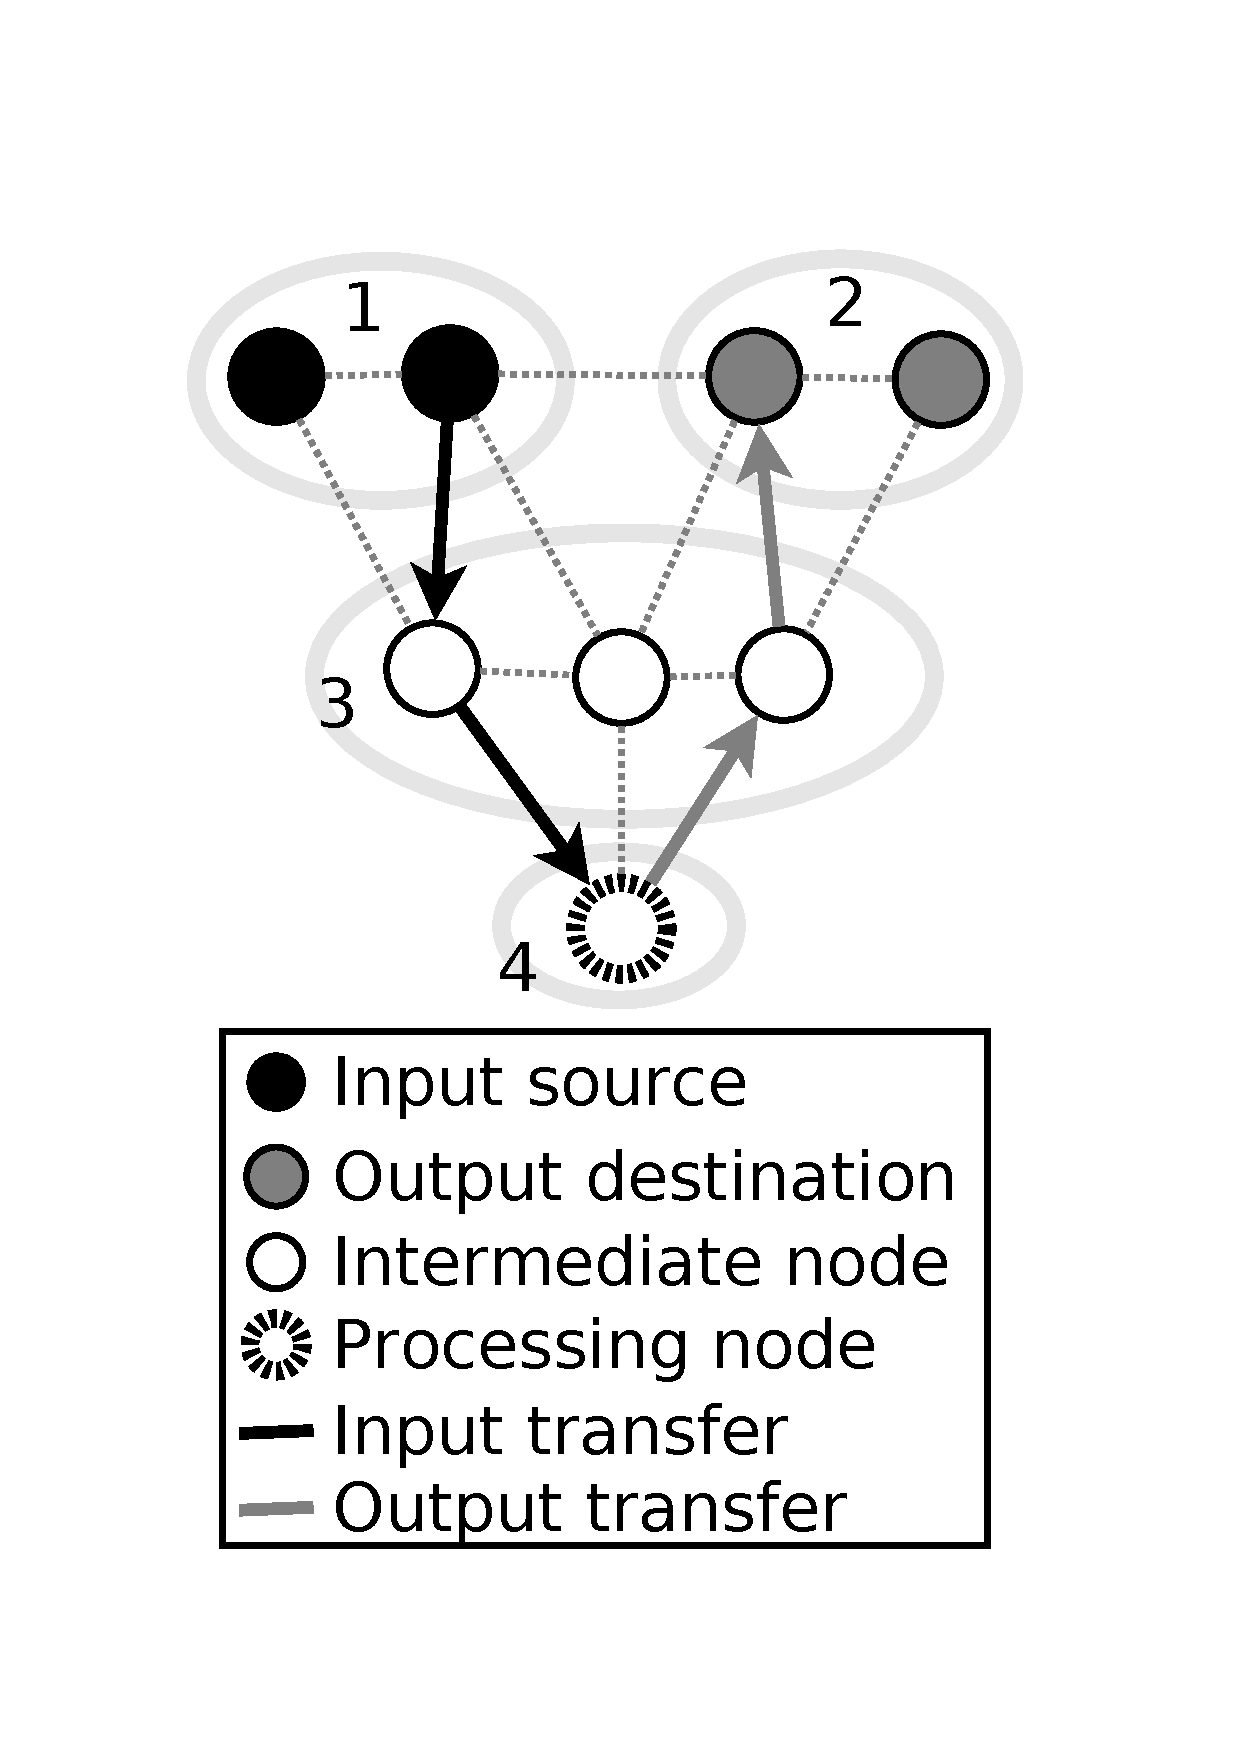
\includegraphics [trim =30mm 35mm 30mm 40mm ,clip, width=.4\textwidth]{pic/link_selection_bw3.pdf}	
    \caption{An example of a transfer path. Illustration for constraints 1-4 in section \ref{path}.  }
    \label{fig:path}
\end{figure}
At the planning stage we have to assign a transfer path for an input and an output file of each job which can be defined by the following constraints (see Figure \ref{fig:path}):
\begin{description}
\label{path}
		%\setcounter{enumi}{-1}
		\item[1.] An input file has to be transferred from one of its sources over exactly one link.
		\item[2.] An output file has to be transferred to one of its destinations over exactly one link.
		\item[3.] An intermediate node (neither source, destination nor selected for the job execution) either has exactly one incoming and outgoing transfer or is not on a transfer path:\\ $\exists$ incoming transfer $\Leftrightarrow \exists$ outgoing transfer. 
		\item[4.] There must exist exactly one incoming transfer of an input file and exactly one outgoing transfer of an output file at the node which was selected for the job execution.	
		\item[5.] A file can be transferred from/to each node at most once.		
\end{description}
In addition, we use constraints for loop elimination similarly as it is described in \cite{Rudova}.

\subsection{Constraints at the scheduling stage}
At the scheduling stage the problem is to assign a start time for each task. The following constraints on order of tasks are implemented:
\begin{itemize}
\item An outgoing transfer of a file from a node can start only after an incoming transfer to that node is finished.  The first transfer of an input file from its source and the first transfer of an output file from the processing node are exceptions from this constraint.
\item A job can start only after the input file is transferred to the selected processing node.
\item An output file can be transferred only after the job is finished.
\item A reservation of space for a file at a node is made when a transfer to that node starts.
\item A file can be deleted from the start node of a link after the transfer is finished.
\item  A reservation of space for an output file is made at the processing node when the job starts.
\item An input file can be deleted from a processing node after the job is finished.
\end{itemize}
Cumulative constraints are widely used in Constraint Programming for description of resource usage by tasks. Each cumulative constraint requires that a set of tasks given by \textit{start times}, \textit{durations} and \textit{resource usage}, never require more than a \textit{resource limit} at any time. In our case we use three sets of cumulative constraints: for CPUs, storages and links (see Table \ref{tab:cumulative}).

\begin{table}
\caption{Variables and parameters used in cumulative constrains on resources.}
\label{tab:cumulative}
\begin{center}
\begin{tabular}{ l  l  l  l  l }
 \hline                   
  Task & Start & Duration & Usage & Limit \\ \hline 
  Job & \textbf{$Js_{jc}$} & $duration_{j}$ & $1$ & $cpu_{c}$ \\ 
  Transfer & \textbf{$Ts_{fl}$} & $size_{f}\cdot slowdown_{l}$ & $1$ & 1 \\ 
  File placement & \textbf{$Fs_{fc}$} & \textbf{$Fdur_{fc}$} & $size_{f}$ & $disk_{c}$ \\ 
  \hline 
\end{tabular}
\end{center}
\end{table}

\subsection{Simulations}
The constraint satisfaction problem was implemented using MiniZinc \cite{MiniZinc} and Gecode \cite{Gecode} was used as a solver. The timelimit was set to 3 minutes for both planning and scheduling stages. The simulations were running under Windows 8 64-bit on a computer with Intel i5 (4 cores) 2.50 GHz processor and 6 GB of memory installed. The Gecode solver was running in a parallel mode using 4 threads. 

%add a schema of the simulation
The simulated environment consisted of 3 nodes: a central storage HPSS ($cpu_{HPSS}=0$) which was the single source for input files and the single destination for output files, a local processing site and a remote processing site. The slowdown of links between the central HPSS and the local site was set to 0, which means that transfer overheads to/from the local site are negligible comparing to a job duration. The slowdown of the links to/from the remote site was increasing in each simulation proportionally to a slowdown factor. The parameters of jobs were taken from logging system of the STAR experiment's data production at computational site KISTI (Korea Institute of Science and Technology Information) \cite{KISTI}. The average job duration was 3,000 minutes and average time of transfer was 5 and 10 minutes to/from the remote site respectively (in the simulations where the slowdown factor $= 1$). Then, in further simulations the transfer times increase proportionally to the slowdown factor. In the simulated environment 80\% of CPUs were available at the local site and 20\% at the remote site. 2,000 of jobs were scheduled stepwise by subsets (chunks) of 200. Storage constraints were not considered in these simulations. Four different scheduling strategies were compared:
\begin{description}
\item[Local:] All the jobs are submitted to the local site only. This strategy was used as a base line for comparison against other strategies.
\item[Equal CPU load:] Jobs are distributed between nodes with the goal to maintain an equal ratio of job duration per CPU. Each input file is transferred prior to the start of a job. At each node jobs are executed in input order.
\item[Data transferred by job:] Each CPU pulls a job from the queue when it is idle, then it has to wait for an input transfer before the job execution starts.
\item[Optimized:] This strategy is based on the model proposed in this paper.
\end{description}


\begin{figure}[h]
    \centering
    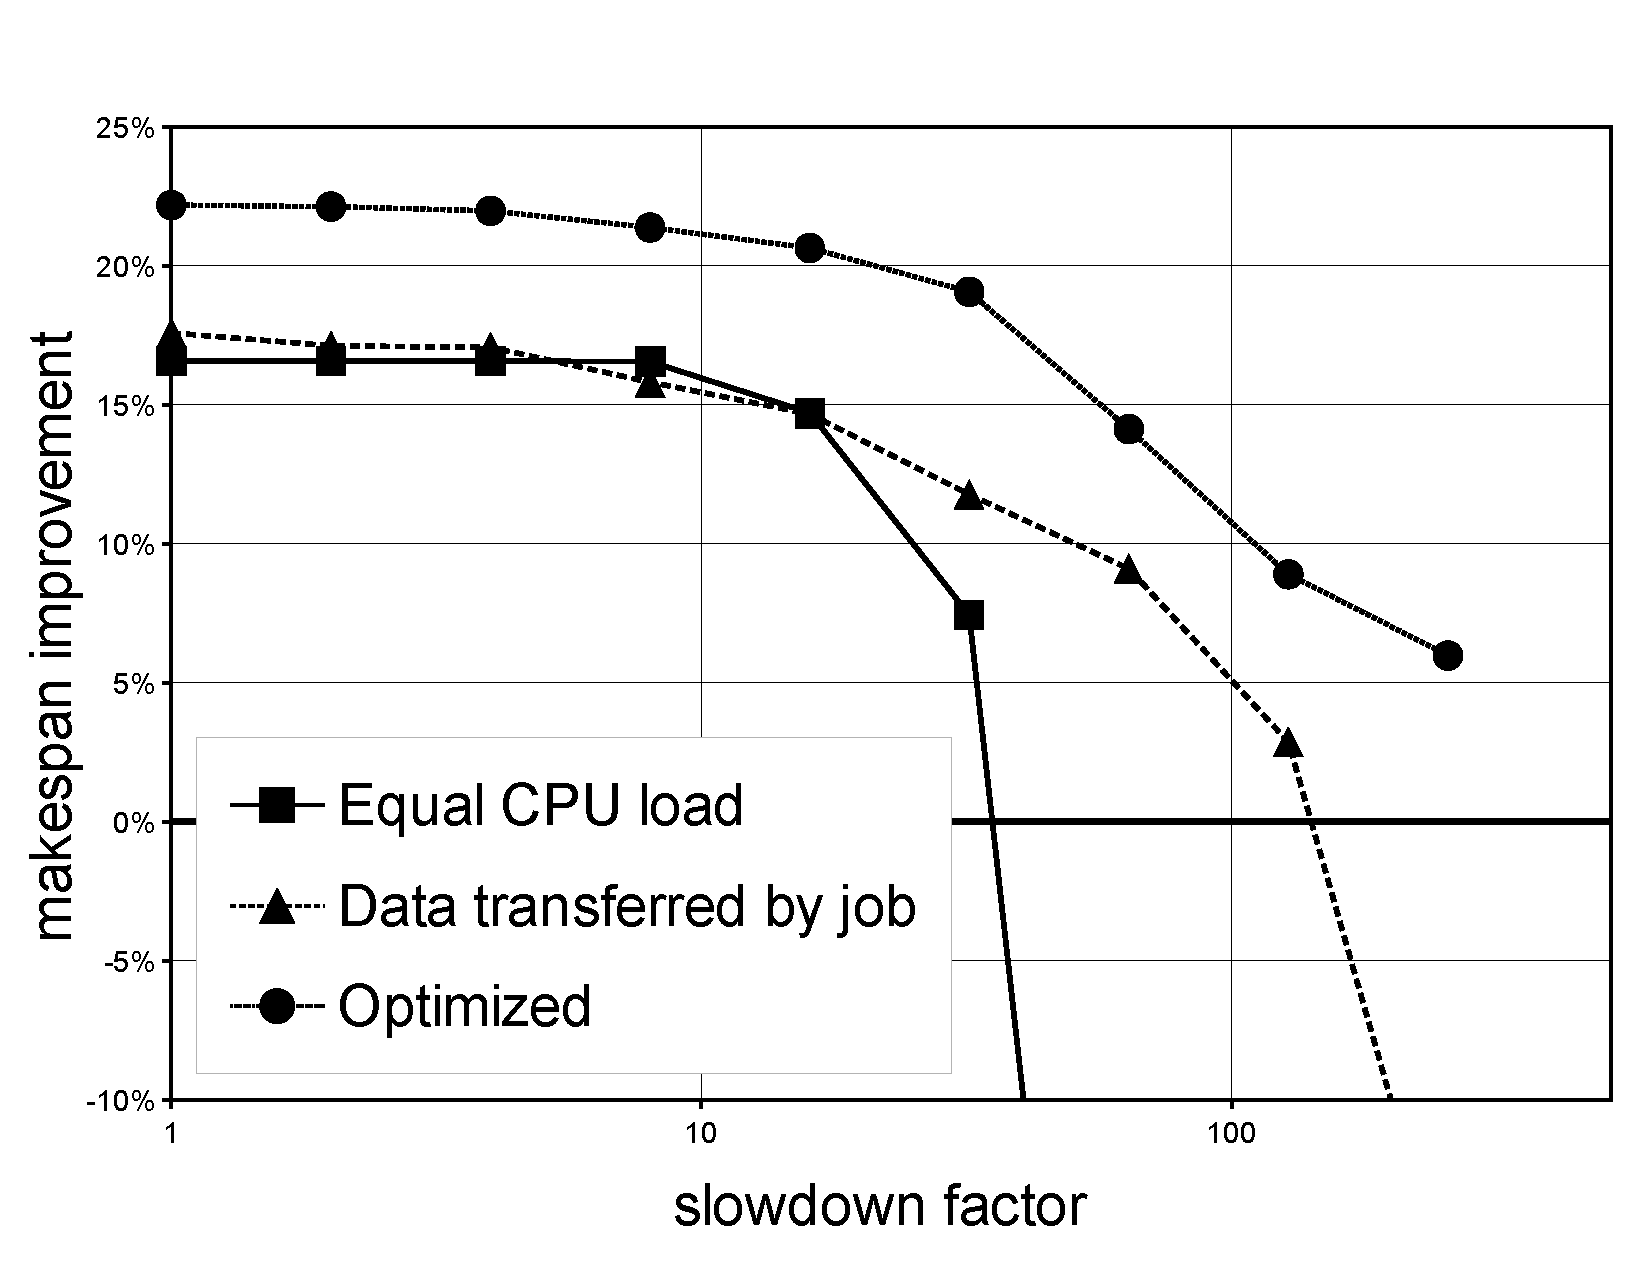
\includegraphics[trim =5mm 5mm 5mm 10mm ,clip,width=0.7\textwidth]{pic/makespan_vs_slowdown4.pdf}
    \caption{Results of simulations for real data production. Three strategies were evaluated and compared to a ideal local production. The
   optimized solution (our model) clearly provides the highest gain.}
    \label{fig:makespan_vs_slowdown}
\end{figure}

The plot at Figure \ref{fig:makespan_vs_slowdown} shows the gain in a makespan delivered by different scheduling policies compared to the job execution at the local site only. The curves show the performance of the scheduling policies when an overhead of transfer to the remote site increases proportionally to the slowdown factor. When the transfer overhead becomes significant both heuristics (``Equal CPU load'' and ``Data transferred by job'') fail to provide an efficient usage of the remote resources (the makespan improvement goes below zero). Negative makespan improvement means that, in this case, it would be faster to process all the data locally than to distribute it between several sites relying on the heuristic. The proposed global planning approach (Optimized) systematically provides a smaller makespan and adapts to the increase of transfer overheads better then the other simulated  heuristics. It was able to provide a positive gain in makespan by using remote resources even when the transfer overhead is comparable to a job duration.  

\section{Enabling caching}
\label{Cache}
Efficient usage of available cache space is important for transferring and accessing data in computational grids. Though, a great variety of caching algorithms is known, a study is needed to evaluate which one can deliver the best performance in data access considering the realistic demand patterns.
 
Cache cleaning algorithms can be applied to keep in the cache of data-transfer tools files that may be reused. The size of those cache is small (several percent of the entire dataset)  and the clean up has to take place regularly to make space for further transfers. Another task can, for example, be to delete a part of local data replica if no longer in use or requested. The problem posed by cache cleanup is to select and delete files which are the least likely to be used again. An investigation to find the most appropriate algorithm is required.

In this study, all the caching algorithm were implemented following the concept known as "water-marking". Water-marking is an approach where  thresholds are set for the cache cleanup starts and stops. It considers the current disk space occupied by the data in cache and the high-mark and the low-mark for cache size are externally set up and can be adjusted as needed. When the used cache size exceeds the high-mark, the cache clean-up starts, and files are deleted until the used cache size gets below the low-mark. The time interval between clean-ups depends on combination of high/low marks, cache size and data-flow. With watermarking concept more computational  demanding algorithms can be implemented as the cleanup may be independent of the data transfers.

\subsection{Access patterns}
Several data  access patterns were extracted from log files of data  management systems  at  sites of HEP/NPP  experiments in order to simulate caching.   Three  different  access patterns were used as input for our simulations:
\begin{itemize}
	\item[]\textbf{STAR1:} the pattern was extracted from Xrootd \cite{Xrootd} logs taken from the STAR experiment's Tier-0 site of RHIC Computing Facility at Brookhaven National Laboratory  (RCF@BNL), it consist of records made during a 3 months period (June-August 2012) of all datasets available in STAR.
	%user analysis access pattern
	\item[]\textbf{STAR2:} extracted from the same data management system, but of records made during a 7 months period (August 2012 - February  2013) under similar conditions.
	%user analysis access pattern
	\item[]\textbf{GOLIAS} farm is part of regional computing center for particle physics at the Institute of Physics (FZU) in Prague, and is part of a Tier-2 site for the CERN/ATLAS experiment. The facility also performs data processing for another experiment - AUGER, which makes less than  1\% of the total requests. The pattern was extracted from DPM \cite{DPM} logs for a 3 months period (November 2012 - February  2013).
	%mixed user analysis and data production access pattern ????
\end{itemize}

The usage of access patterns corresponding to different time periods and experiments helps to verify the results of our simulations. As input of our simulations, we tried to focus on a few characteristic access patter. The key parameters we came up with for the three access patterns are given in Table \ref{patterns}. Both STAR access patterns have similar parameters. It is noteworthy to mention that the first one was taken right before the Quark Matter 2012 conference and the second one, right after. This is important as the access to data is intensified before a conference and without verification, it would be doubtful if our findings would be stable across time. The  number  of files requested  only once during  the period, is less than  10\% in both cases. 

The FZU/GOLIAS access pattern is taken from another experiment with different data-storage structure, DPM is used here within a Tier-2 data access context (user analysis). This access pattern is much less uniform and differs from the other  two:  the size of files is not explicitly limited and can reach 18 GB, the number of requests for a file varies from 1 up to 94260, with an average 5, while it varies from 1 to 203 for the STAR patterns. 44\% of files were requested  only once

Our analysis is not sensitive to the particular Data Management system, (Xrootd or DPM), further we explain  differences in the access patterns with specifics of experiment and role of the cluster in the system (tier level).


\begin{centering}
\begin{table}
\caption{Summary of three user access patterns used as input for simulations. The selection of two time sequence in STAR and one from a different experiment aims at verifying stability of our result and findings.}
\centering
\begin{tabular}{lllll}
\hline
 &  &STAR1 & STAR2  & GOLIAS  \\ \hline
Time period& months & 3 & 7 & 3 \\ 
Number of requests&$ \times 10^{6} $& 33 & 52 & 21 \\ 
Data transferred& $ PB $ & 50 & 80 & 10 \\ 
Maximal number of requests for one file& $- $ &  192 & 203  & 94260 \\ 
Average number of requests per file& $- $ & 19 & 15 & 5 \\ 
Number of unique files& $\times 10^{6} $ & 1.8 & 1.7  & 3.8 \\ 
Total size of dataset& $PB $ & 1.45 & 2 & 1 \\
Maximal file size & $GB $ & 5.3 & 5.3 & 18 \\ 
Average file size & $ GB $& 0.8 & 1  & 0.3 \\ 	
\hline
\end{tabular}	
\label{patterns}
\end{table}
\end{centering}


\subsection{Cache simulation}
The efficiency of caching can be estimated by two quantities, the cache hits $H$ and cache hits per megabyte of data $H_{d}$ from here on referred to as \textit{cache data hits}:

\begin{equation}
\label{hits}
H =\frac{N_{cache}}{N_{req}-N_{set}}
\end{equation}

\begin{equation}
\label{hitsBeq}
H_{d} = \frac{S_{cache}}{S_{req}-S_{set}}
\end{equation}
where $N_{req}$ is the total number of requests, $S_{req}$ -the total amount of transferred data in bytes, $N_{set}$ -the number of unique files witch were requested at least ones during the considered period, $S_{set}$ - the total size of those unique files in bytes, $N_{cache}$ - the number of files transferred from cache, $S_{cache}$ - the amount of data transferred from cache in bytes.

By maximizing the cache hits $H$ one reduces the number of files transferred from external sources and thus reduces the overall make-span due to transfer startup overhead for each file. By maximizing the cache data hits $H_{d}$ one reduces the network load, since more data is reused from the local cache.

If the access pattern is completely random, the expected cache hit and cache data hits would be equal to $cache~size/storage~size$, so it can be useful to compare the actual cache performance to this estimation. 

Altogether 27 different caching algorithms were simulated. But the majority of studied algorithms did not bring any improvements over the simplest one (FIFO). Only the algorithms that appeared to be the most efficient are discussed below: 
\begin{itemize}
\item[\textbf{-}]\textbf{First-In-First-Out (FIFO)}: evicts files in the same order they entered the cache. Performance of this trivial algorithm  provide a good comparison benchmark against  more sophisticated ones  which can demand  significant computational resources.
\item[$\bigcirc $]\textbf{Least-Recently-Used (LRU)}: evicts the set of files which were not used for the longest period of time.
\item[\begin{Large}$\bullet $\end{Large}]\textbf{Least-Frequently-Used (LFU)}: evicts the set of files which were requested less times since they entered the cache.
\item[$\bigstar $] \textbf{Most Size (MS)}: evicts the set of files which have the largest size.
\item[\textbf{+}]\textbf{Adaptive Replacement Cache (ARC)}\cite{ARC}: splits cached files into two lists: L1 - files with $access~count=1$, and L2 - files with $access~count>1$. LRU is then applied to both list, the self adjustable parameter $p = cache~hits~in~L1 / cache~hits~in~L2$ defines the number of cached files in each list. The general idea is to invest more into the list which delivers more hits.
\item[$\ast $]{\textbf{Least Value based on Caching Time (LVCT)}}\cite{Cache_in_Grid}: Deletes files with the smallest value of the  Utility Function:
\begin{equation}
Utility Function = \frac{1}{Caching Time \times File Size}
\end{equation}   
where \textbf{Caching Time} of a file F is total size of all files accessed after the last request for the file F.
\item[$\bigtriangledown $]{\textbf{Improved-Least Value based on Caching Time (ILVCT)}}\cite{ILVCT}: Deletes files with the smallest value of the  Utility Function:
\begin{equation}
Utility Function = \frac{1}{Number Of Accessed Files \times Caching Time \times File Size}
\end{equation}   
where \textbf{Caching Time} is the same as for LVCT and \textbf{Number Of Accessed Files}  is a number of files requested after the last request for selected file. 
\end{itemize}


\subsection{Simulation results}
Three series of simulations with three access patterns were performed for each algorithm (90 simulations in total for each algorithm): 
\begin{itemize}
\item 10 simulations with cache size 1-90 \% of storage with fixed low-mark 75\% and high-mark 95\%. Those simulations aim to understand what would happen if we have to periodically clean a large storage. Those cases are aligned with a DPM and Xrootd use where most (if not all) the dataset(s) are in the system.
\item 10 simulations with cache size 1.2 - 0.0025\% of storage with fixed low-mark 75\% and high-mark 85\%. This high-mark was selected in order to leave enough margin (15\%) in case when a large file is requested at the moment when the cache is almost full. We used those simulations to understand the behavior of cache cleanup if the cache size is by several orders less than the dataset size. This is in fact a most common case for transfer cache on data transfer nodes.
\item 10 simulations with fixed cache size 10\% of storage,fixed high-mark 95\% and  variable low mark  within 0-90\%. We performed those simulations to better understand the effect of data retention on cache (delete the least in hope of re-use).
\end{itemize}

In order to compare one algorithm against another an average improvement can be calculated in a following way:
\begin{equation}
Average~improvement = \frac{\sum^{n}_{i=1}\frac{value2_{i}-value1_{i}}{value1_{i}}}{n},
\end{equation}
where $n$ is the total amount of simulations with equal parameters for both algorithms, $i$ is the number of the simulation,$value1$ - cache hits or cache data hits of a reference algorithm (FIFO), $value2$ - cache hits or cache data hits of a compared algorithm.

Table \ref{results} contains the results of comparison of all the algorithms represented in this paper against FIFO. 60 values for each algorithm were taken from results of simulation series 1 and 2 in order to calculate the average improvement. According our results, the LFU algorithm does not bring any improvement over FIFO due to its well known flaw - it accumulates files which were popular for a short period of time, and those files prevent newer ones from staying in cache. The ARC algorithm was developed as an improvement to LRU, and not surprisingly, it outperforms LRU by $\sim$5\% in cache hits and $\sim$7\% in cache data hits. Therefore, LFU and LRU algorithms could be excluded from the further analysis in our case studies.

The graphical detailed results of simulations for all 3 series are given at Figures \ref{plots:big}-\ref{plots:low}. The performance of FIFO and 3 algorithms appeared to be the most efficient (MS, ACR and LVCT) is presented at the plots. 

Difference between Tier-2 and Tier-0 access patterns leads to distinct cache performance. Only the data dedicated for the ongoing analysis is placed at the Tier-2 site, while at the Tier-0 site all the experimental data is stored. As a result -- the access pattern at the Tier-2 site has stronger access locality. STAR1 and STAR2 access patterns correspond to Tier-0 site and GOLIAS to a Tier-2 site.  Thus, any particular algorithm at the plots delivers higher cache hits and cache data hits for GOLIAS access pattern than for STAR1 and STAR2.  


The behavior of algorithms is similar within each dataset that is, their respective performance ordering is the same. This observation implies that if one of the algorithm appears to be most efficient for one of the datasets it is also the most efficient for the other datasets. This statement is also true for the rest of simulated algorithms not present on our figure. Though the communities represented by the STAR and GOLIAS access patterns are somewhat similar, this result is slightly surprising as our case studies represent two time sequence within the same usage and totally uncorrelated experiments. It would be interesting to study those algorithms in a different experimental context (outside the HEP/NPP communities) but this study is outside the scope of our research. 

The MS algorithm has shown outstanding cache hits, but the lowest cache data hits. At the same time the LVCT has cache hits comparable to the MS while cache data hits are 2\% improved over the FIFO. This algorithm could be an optimal when the cache hits is the target optimization parameter. The ARC algorithm has shown the highest cache data hits for studied access patterns.

The dependence of algorithms performance on low mark is presented at Figure \ref{plots:low}. With higher low mark the number of clean-ups increases and that is why the difference between algorithms becomes more notable. Performance of efficient algorithms (FIFO, LRU, ARC and LVCT) increases steadily with the low mark. One should be careful when setting up a cache low mark at a particular site, since a higher low mark can increase cache performance significantly, but at the same time it can result in running cache clean-ups too often, consuming significant computational resources (and potentially increasing the chance to interfere with data transfers hence, degrading transfer performances if delete/writes/read overlap).

        \begin{figure}
                \centering
                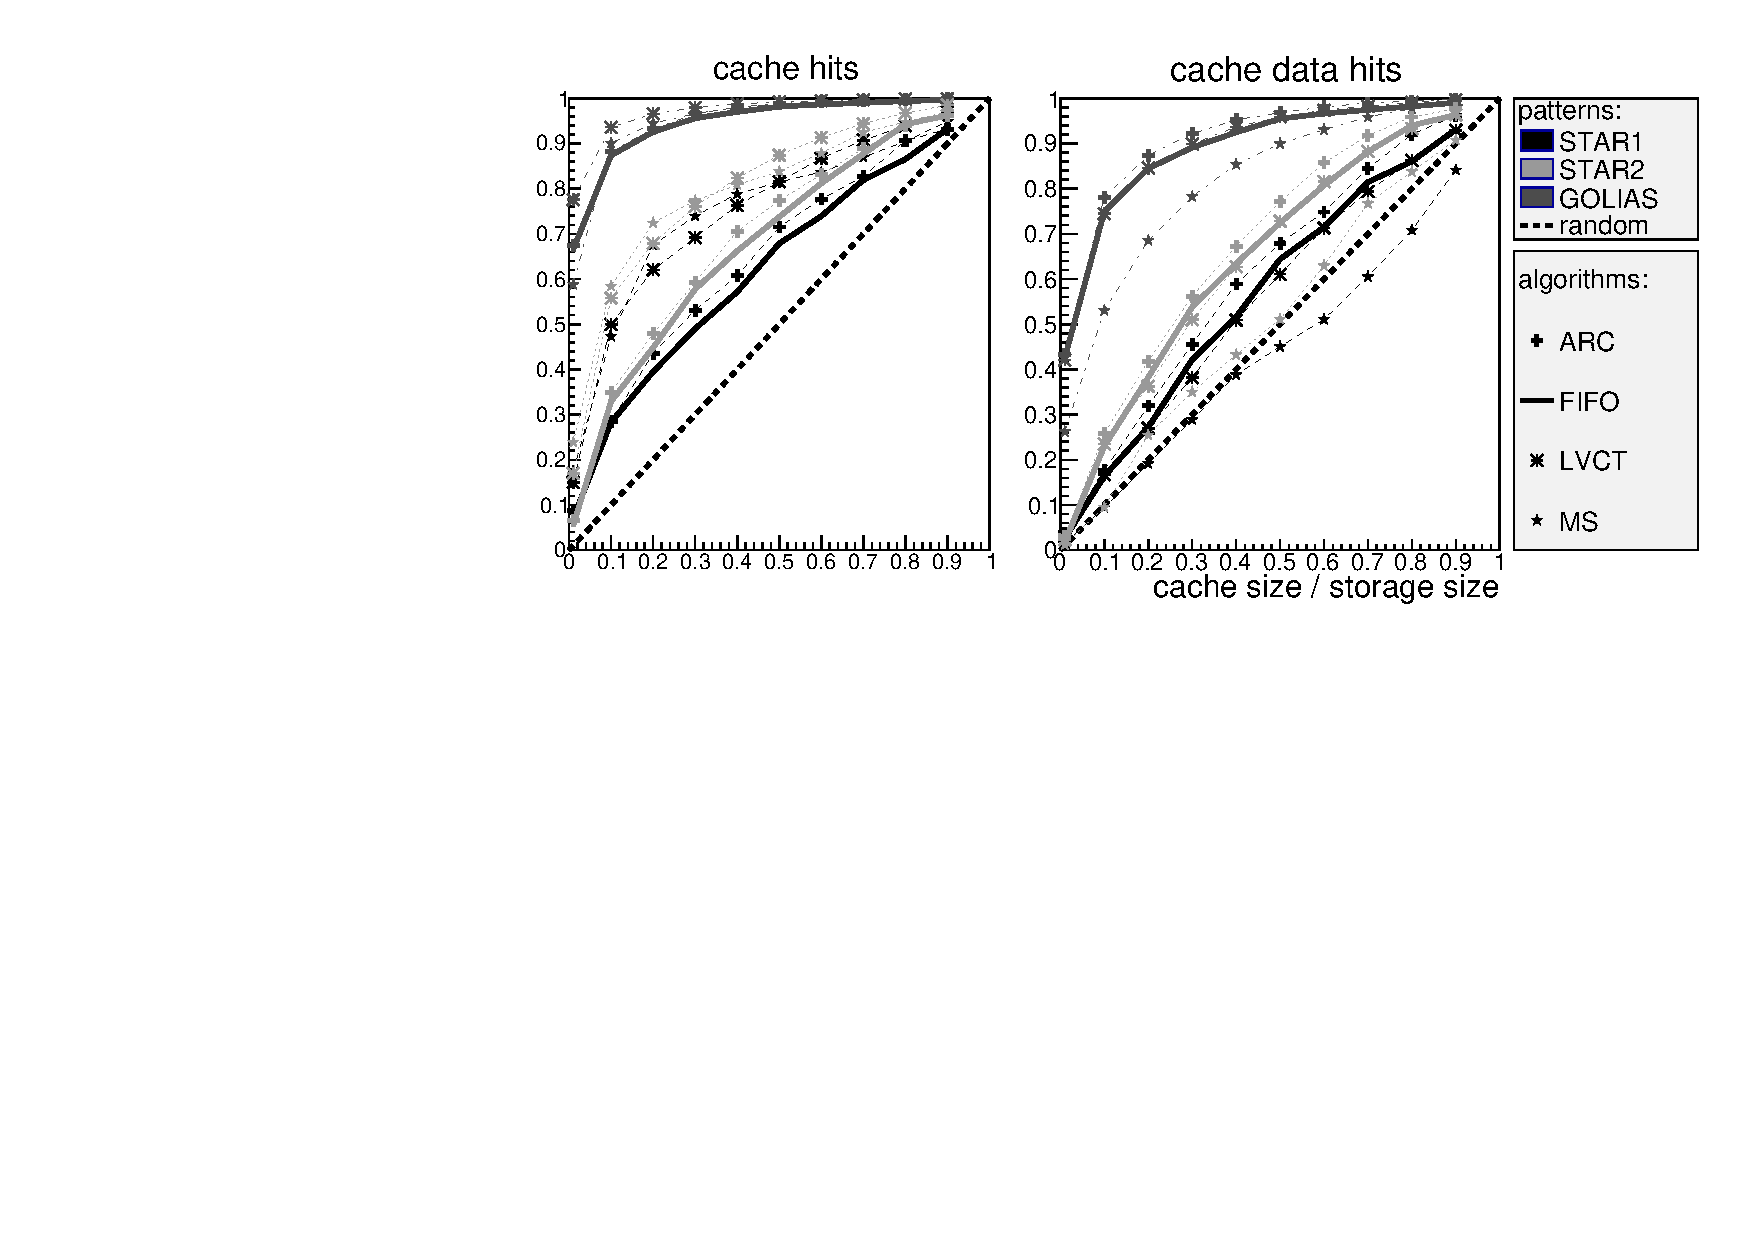
\includegraphics[width=\textwidth, natwidth=610,natheight=642]{pic/big-basic.pdf}
                \caption{Results of simulation. Performance of algorithms for cache of larger size can be compared. For all of the simulations on this plot the following parameters were fixed: low mark = 0.75, high mark = 0.95 }
                \label{plots:big}
        \end{figure}%

        \begin{figure}
                \centering
                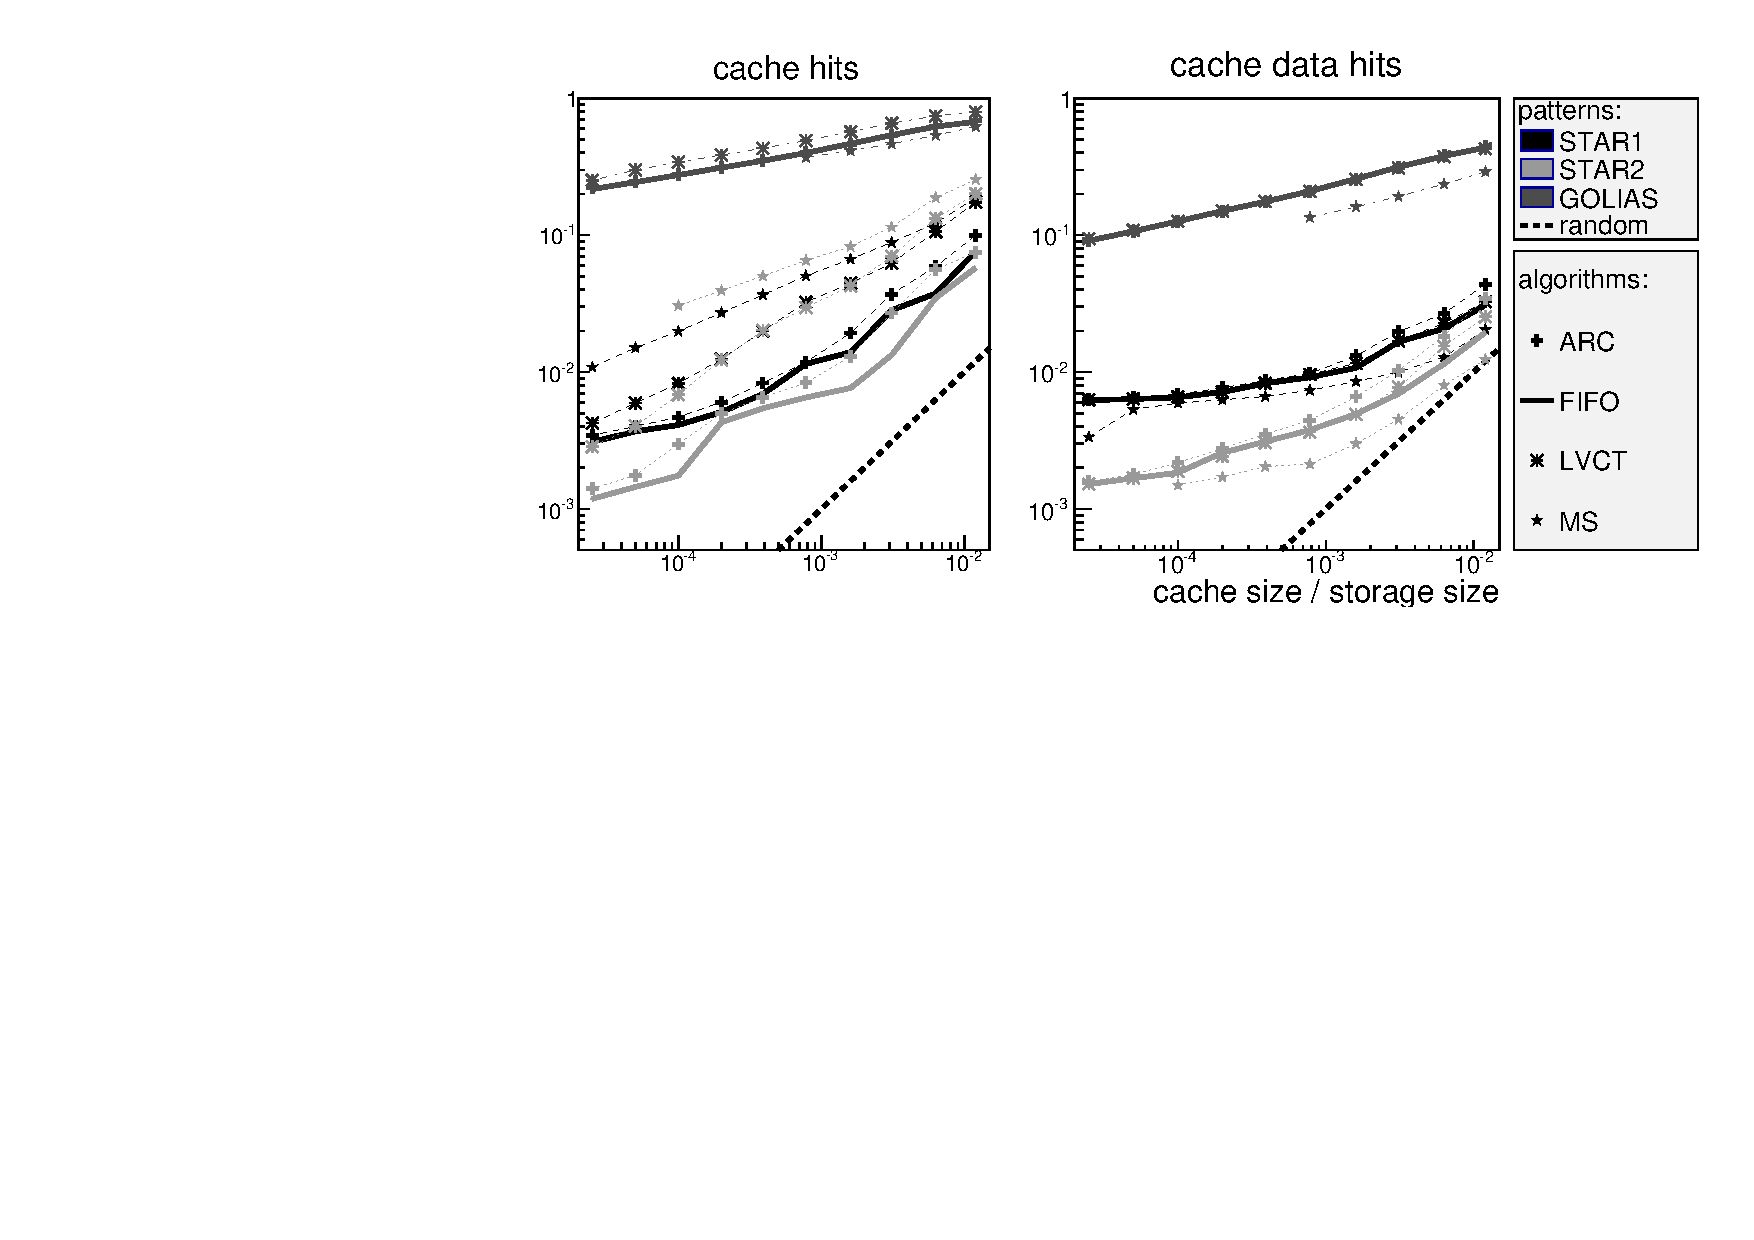
\includegraphics[width=\textwidth, natwidth=610,natheight=642]{pic/tiny-basic.pdf}
                \caption{Results of simulation. Performance of algorithms for cache of smaller size can be compared. For all of the simulations on this plot the following parameters were fixed: low mark = 0.75, high mark = 0.85}
                \label{plots:tiny}
        \end{figure}

        \begin{figure}
                \centering
                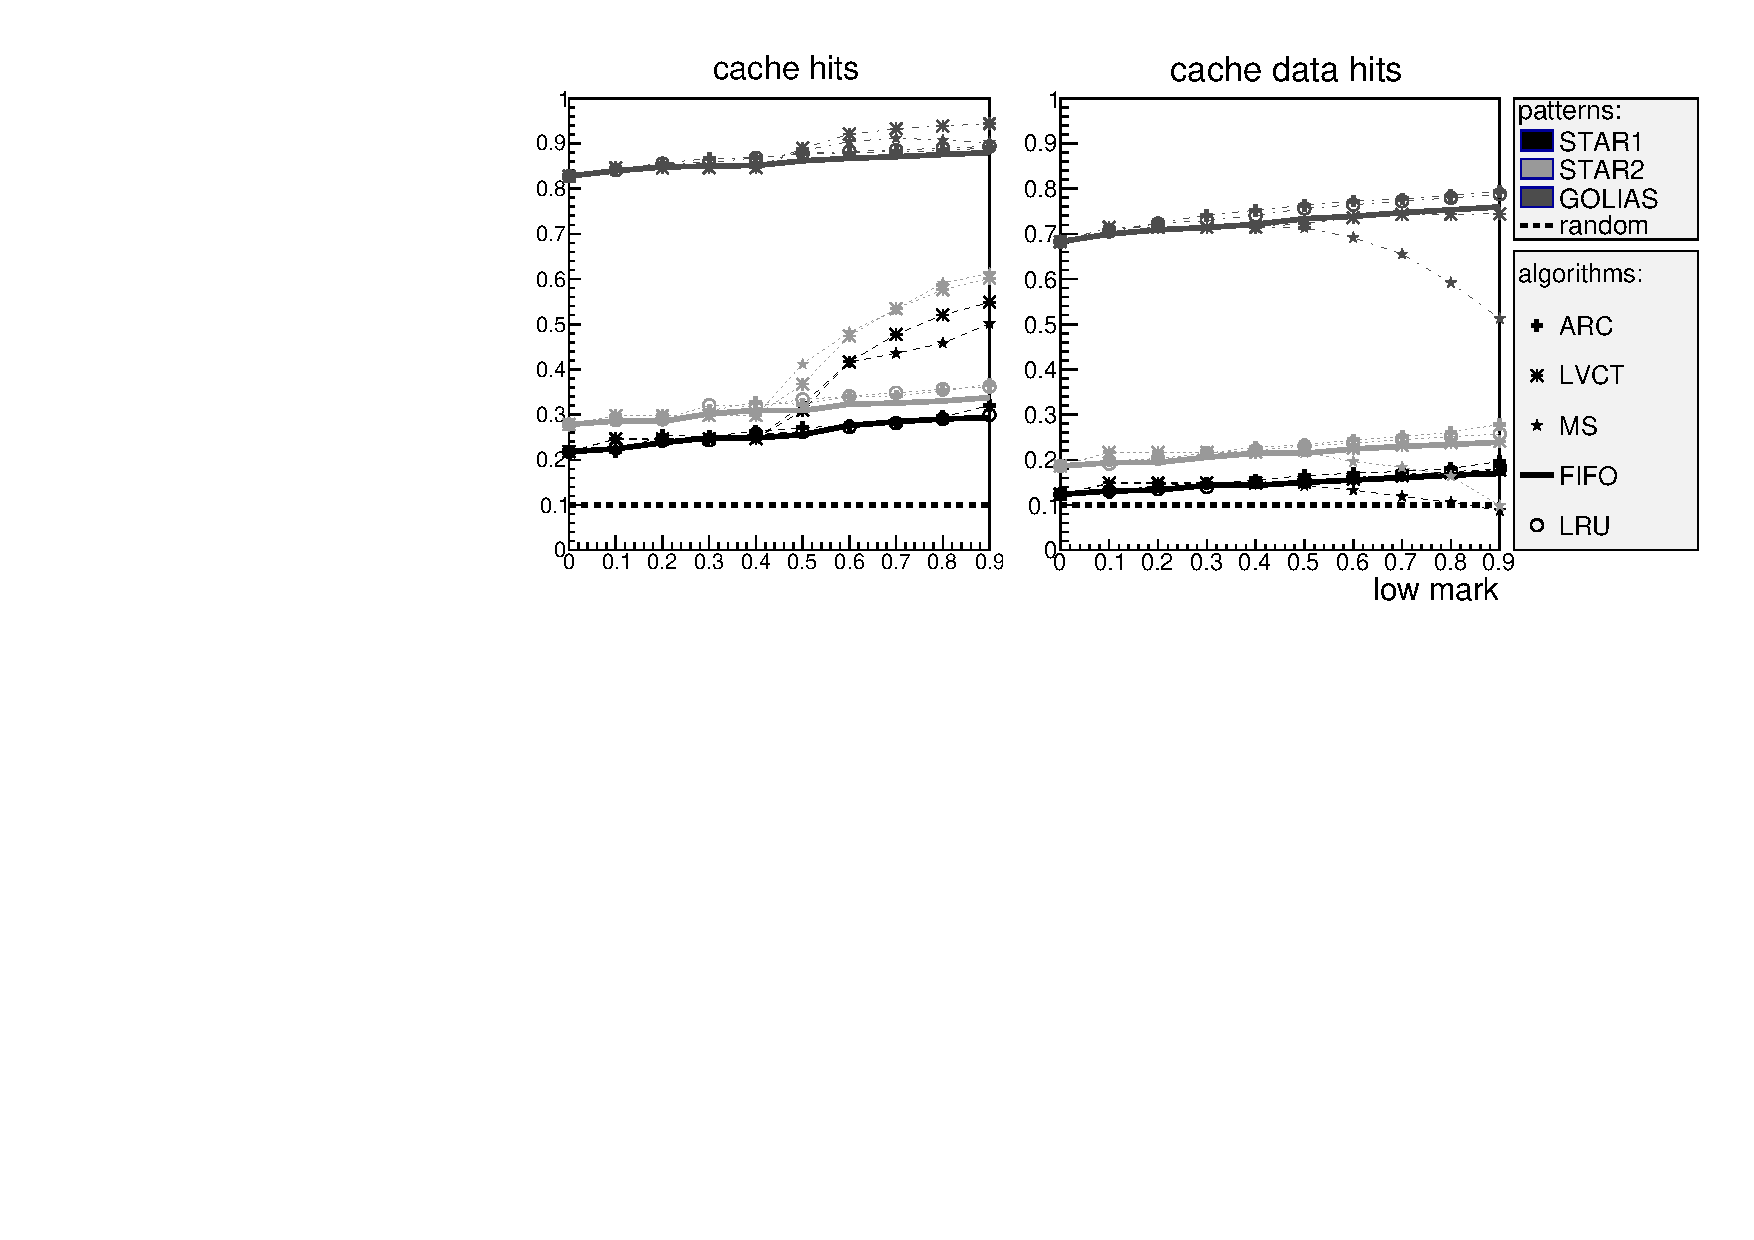
\includegraphics[width=\textwidth, natwidth=610,natheight=642]{pic/low-basic.pdf}
                \caption{Results of simulation: dependence of cache performance on low mark. For all of the simulations on this plot the following parameters were fixed: cache size / storage size = 0.1, high mark = 0.95}
                \label{plots:low}
        \end{figure}


\begin{table}
\caption{Average improvement of algorithms over FIFO.}
\centering
\begin{tabular}{lrr}
\hline
Algorithm & cache hits & cache data hits\\ \hline
MS & \textbf{116} \% & -20 \% \\ 
LRU & 8 \% & 5 \% \\ 
LFU & -27 \% & -18 \% \\ 
ARC & 13 \% & \textbf{11} \%\\ 
LVCT & \textbf{86} \%& 2 \%\\ 
ILVCT & \ 28 \%& 2 \%\\ 
\hline
\end{tabular}	

\label{results}
\end{table}


\subsection{Selection of a caching policy}
Performance of cache algorithms implemented with watermarking concept was simulated for a wide range of cache sizes and low marks. Three access patterns from Tier-0 and Tier-2 sites of 2 different experiments were used as input for simulations.
Regardless of the cache size, Tier-level and specificity of experiment the LVCT and ARC appeared to be the most efficient  caching algorithms for the communities we investigated. While we found the stability of relative  algorithms' performance surprising at first, we attribute this result to an access pattern which is intrinsically similar in nature.
An extension of this work could be the investigation of this result in a different experiment context which is a work beyond our initial goal. LVCT and ARC could certainly be safely implemented in tools such as RIFT.
\begin{itemize}
	\item If the goal is to minimize makespan due to a transfer startup overhead the LVCT algorithm should be selected.
	\item If the goal is to minimize the network load the ARC algorithm is an option.
\end{itemize}



\section{Conclusion and future plans}
Distributed data processing in HENP as well as other data intensive applications for Grid require further improvement of load planning and job scheduling. Inspired by success of global planning for distributed systems \cite{Zerola} and media streams \cite{Rudova} we extended these approaches to the entire data production in HENP, combining job scheduling and data management.  

In Section \ref{Network_flow} we proposed a model of distributed data production, where all the files from a single source has to be processed once and transferred back. This model allows planning of WAN, storage and CPU loads using the network flow maximization approach. 

In Section \ref{CP_approach} a model for scheduling of data production over Grid was formulated in form of constraint satisfaction problem and solved using constraint programming. The simulations based on data extracted from log files of batch and data management systems of the STAR experiment has shown that the proposed global planning approach systematically provides a smaller makespan and adapts to the increase of transfer overheads better then the other simulated  heuristics.

Both described approaches can be combined in a two-stage scheduling. At the first stage the load of the resources will be planned using the network flow maximization problem knowing the current state of the Grid. At this point the amount of data that should be transferred over each link and processed at each site will be calculated. Then, at the second stage, particular file transfers and jobs will be scheduled using our constraint programming model. 

In addition to planning of data production, caching algorithms for user analysis were studied. The most widely used known algorithms were compared in multiple series of simulations using data access patterns extracted from log systems of two distinct experiments. Two best performing algorithms were selected to be used for cache management in HENP computational Grids. 

The achieved results will be used in a distributed data production planner which is being developed. The planner will enable automated and scalable planning and optimization of distributed computations which are highly required in data intensive computational fields such as High Energy and Nuclear Physics.

The future development of global planning for data processing in Grid is ongoing. In future we plan to:
combine both proposed approaches in a global scheduler;
test this approach using full scale Grid simulations with the help of modeling tools widely used in Grid research community;
improve the planner performance in order to enable online scheduling in real environment. 


\section*{Acknowledgements}
This work has been supported by the Czech Science Foundation
(13-20841S, P202$/$12$/$0306),  the MEYS grant CZ.1.07/2.3.00/20.0207 of the European Social Fund (ESF) in the Czech Republic: “Education for Competitiveness Operational Programme” (ECOP) and the Office of Nuclear Physics within the U.S. Department of Energy.  




%\bibliography{bibliography}{}
%\bibliographystyle{spmpsci}

%\begin{refsection}
%\nocite{ACAT_2014}
%\printbibliography[heading=Publications]
%\end{refsection}

\printbibliography

		

\end{document}
